\documentclass[11pt, a4paper, oneside]{Thesis}
\usepackage{floatrow}
\floatsetup[table]{capposition=top}
\usepackage{textcomp}
\usepackage{wrapfig}
\usepackage{lscape}
\usepackage{rotating}
\usepackage{graphicx}
\usepackage{caption}
\usepackage{amsmath}
\usepackage{upgreek}
\usepackage{subcaption}
\usepackage{gensymb}
\usepackage{csquotes}
\usepackage{pdfpages}
\usepackage{lipsum}
\usepackage{xcolor}
\usepackage{algorithm}
\usepackage{algpseudocode}
% Allow hyphenation in monospace font and fix quotes in listings
\usepackage[T1]{fontenc}
\usepackage{upquote}
\usepackage{tikz}
\usetikzlibrary{shapes.geometric, arrows.meta, positioning, fit, backgrounds, calc, decorations.pathreplacing}
\usepackage{listings}
\lstset{
  basicstyle=\ttfamily\small,
  breaklines=true,
  frame=single,
  backgroundcolor=\color{gray!8},
  keywordstyle=\color{blue!70},
  commentstyle=\color{green!50!black},
  stringstyle=\color{orange!80!black},
  numbers=left,
  numberstyle=\tiny\color{gray},
  numbersep=5pt
}
\usepackage{booktabs}
\usepackage{multirow}
\usepackage{url}
\usepackage{xurl}
\usepackage{acronym}
\usepackage{array}
\newcolumntype{L}{>{\centering\arraybackslash}m{3cm}}

\makeatletter
\AtBeginDocument{%
  \renewcommand*{\AC@hyperlink}[2]{%
    \begingroup
      \hypersetup{hidelinks}%
      \hyperlink{#1}{#2}%
    \endgroup
  }%
}
\makeatother

\graphicspath{{Pictures/}}
\usepackage[numbers, sort&compress]{natbib}

\hypersetup{urlcolor=black, colorlinks=true}
\title{\ttitle}

\begin{document}
\makeatletter
\makeatother

\frontmatter

\setstretch{1.6}

\fancyhead{}
\rhead{\thepage}

\pagestyle{fancy}

\newcommand{\HRule}{\rule{\linewidth}{0.5mm}}

\hypersetup{pdftitle={\ttitle}}
\hypersetup{pdfsubject=\subjectname}
\hypersetup{pdfauthor=\authornames}
\hypersetup{pdfkeywords=\keywordnames}

%----------------------------------------------------------------------------------------
%	TITLE PAGE
%----------------------------------------------------------------------------------------

\begin{titlepage}
\begin{center}

\HRule \\[0.3cm]
{\huge \bfseries \ttitle}\\[0.3cm]
\HRule \\[0.8cm]

\large \textit{A thesis submitted in fulfilment of the requirements for the degree of}\\[0.15cm]
\textbf{\degreename}\\[0.2cm]
\textit{by}\\[0.2cm]
\textbf{\authornames}\\[0.2cm]
\textit{under the supervision of}\\[0.15cm]
\textbf{\supnameA}\\[0.15cm]
\textit{Co-advisors:}\\[0.1cm]
\textbf{Dr.\ Yogesh K. Meena} \quad \textbf{Dr.\ Nipun Batra}

\vfill


\includegraphics[width=0.28\linewidth]{Pictures/IITGN.png}\\[0.35cm]
\MakeUppercase\DEPTNAME\\[0.2cm]
\textsc{\MakeUppercase\UNIVNAME}\\[0.3cm]
\large \today

\end{center}
\end{titlepage}

%----------------------------------------------------------------------------------------
%	DECLARATION PAGE
%----------------------------------------------------------------------------------------

\Declaration{\addtocontents{toc}{\vspace{1em}}}
\setcounter{page}{2}

\begin{minipage}{\textwidth}
    It is certified that the work contained in this thesis entitled \textbf{\enquote{\ttitle}} by \textbf{\authornames} \textbf{(\rollno)} has been carried out under my supervision and that it has not been submitted elsewhere for a degree.
\end{minipage}

\vspace{20.00mm}

\begin{minipage}{0.45\textwidth}
\begin{flushleft}
    \textbf{\supnameA}\\
    Professor\\
    Dept.\ of Computer Science \& Engineering\\
    \univname
\end{flushleft}
\end{minipage}
\hfill
\begin{minipage}{0.45\textwidth}
\begin{flushright}
    \textbf{Dr.\ Yogesh K. Meena}\\
    Assistant Professor\\
    Dept.\ of Computer Science \& Engineering\\
    \univname\\[0.6cm]
    \textbf{Dr.\ Nipun Batra}\\
    Associate Professor\\
    Dept.\ of Computer Science \& Engineering\\
    \univname
\end{flushright}
\end{minipage}

\vfill

\clearpage

%----------------------------------------------------------------------------------------
%	ABSTRACT PAGE
%----------------------------------------------------------------------------------------

\abstract{\addtocontents{toc}{\vspace{1em}}

Depression is a pervasive mental health challenge in higher education, where academic pressure, career uncertainty, and social stressors disproportionately affect students. Traditional diagnostic approaches are limited in scalability and often stigmatising, necessitating automated, non-invasive, and interpretable screening tools. This thesis presents a complete system for depression detection from speech via machine learning, deployed as a mobile health (mHealth) platform for proactive screening of university students.

The work spans two interconnected technical threads. First, a series of Speech Emotion Recognition (SER) experiments were conducted as preliminary groundwork, exploring custom feature engineering (pause-histogram and mel-spectrogram features) combined with deep neural network architectures — including 2D CNN with Squeeze-and-Excitation blocks, 1D CNN + LSTM, and 2D CNN + BiGRU — evaluated on RAVDESS, CREMA-D, EMO-DB, TESS, and IESC. These experiments informed feature design choices for the downstream depression detection task.

Second, a complete depression detection pipeline was implemented and evaluated on the DAIC-WOZ corpus. Audio recordings are preprocessed (participant speech extraction and silence removal), segmented into fixed-length windows, and processed by the Time Series Feature Extraction Library (TSFEL) to produce 156 features per segment. Four statistical aggregators (mean, standard deviation, minimum, maximum) yield a 624-dimensional feature vector, fed into a Random Forest classifier (200 trees). Extensive ablation studies across five segment lengths (3, 5, 7, 9, 11 seconds) and four classification thresholds (0.3, 0.4, 0.5, 0.6) identify 7-second segments at threshold 0.5 as the optimal configuration, achieving a macro-F1 of 0.385.

The pipeline is operationalised within a microservices mHealth system comprising a Twilio-based Interactive Voice Response (IVR) module for automated outbound voice data collection, a FastAPI backend, a Celery + RabbitMQ asynchronous task queue, MinIO object storage for secure audio archival, a PostgreSQL relational database, and a React counsellor dashboard. The system is designed around seven principles including scalability, interpretability, and a human-in-the-loop philosophy in which machine learning predictions serve as decision support for trained counsellors.

}

%----------------------------------------------------------------------------------------
%	ACKNOWLEDGEMENTS
%----------------------------------------------------------------------------------------

\clearpage
\setstretch{1.3}

\acknowledgements{\addtocontents{toc}{\vspace{1em}}

I would like to express my deepest gratitude to my supervisor, \textbf{Dr.\ Rajat Moona}, for his invaluable guidance, strategic vision, and unwavering support throughout this research. His insights shaped the direction of this work in fundamental ways.

I am equally thankful to my co-advisors, \textbf{Dr.\ Yogesh K. Meena} and \textbf{Dr.\ Nipun Batra}, for their detailed technical feedback, patient mentorship, and for consistently pushing the quality of this work higher. Their complementary expertise in human-computer interaction and machine learning was indispensable.

I extend my sincere thanks to the Indian Institute of Technology Gandhinagar for providing an outstanding research environment, computational resources, and financial support that made this work possible.

I am deeply thankful to the student volunteers who participated in the pilot study and data collection, and who generously shared their experiences regarding mental health and technology acceptance. I also extend my sincere appreciation to the counselling team at IIT Gandhinagar, whose insights into institutional mental health practice informed the design of the system and whose support was invaluable in shaping a tool aligned with real counselling needs.

Finally, I am profoundly grateful to my family for their unconditional love, patience, and belief in me throughout this journey.

\textbf{\authornames}

}
\clearpage

%----------------------------------------------------------------------------------------
%	LIST OF CONTENTS/FIGURES/TABLES
%----------------------------------------------------------------------------------------

\pagestyle{fancy}
\tableofcontents
\listoffigures
\listoftables

%----------------------------------------------------------------------------------------
%	ABBREVIATIONS
%----------------------------------------------------------------------------------------

\clearpage

\setstretch{1.5}

\chapter*{Abbreviations}
\addtotoc{Abbreviations}
\begin{acronym}
\acro{AI}{Artificial Intelligence}
\acro{API}{Application Programming Interface}
\acro{ASR}{Automatic Speech Recognition}
\acro{AVEC}{Audio/Visual Emotion Challenge}
\acro{BCI}{Brain-Computer Interface}
\acro{CRUD}{Create, Read, Update, Delete}
\acro{CNN}{Convolutional Neural Network}
\acro{DB}{Database}
\acro{DG}{Design Goal}
\acro{EATD}{Emotional Audio-Textual Depression Corpus}
\acro{EEG}{Electroencephalogram}
\acro{F0}{Fundamental Frequency}
\acro{FastAPI}{Fast Application Programming Interface (Python web framework)}
\acro{GRU}{Gated Recurrent Unit}
\acro{HCI}{Human-Computer Interaction}
\acro{HNR}{Harmonics-to-Noise Ratio}
\acro{HTTP}{HyperText Transfer Protocol}
\acro{HTTPS}{HyperText Transfer Protocol Secure}
\acro{IVR}{Interactive Voice Response}
\acro{JWT}{JSON Web Token}
\acro{LIME}{Local Interpretable Model-Agnostic Explanations}
\acro{LSTM}{Long Short-Term Memory}
\acro{MADRS}{Montgomery–Åsberg Depression Rating Scale}
\acro{MFCC}{Mel-Frequency Cepstral Coefficient}
\acro{mHealth}{Mobile Health}
\acro{ML}{Machine Learning}
\acro{MUI}{Material User Interface}
\acro{NLP}{Natural Language Processing}
\acro{ORM}{Object-Relational Mapping}
\acro{PHQ}{Patient Health Questionnaire}
\acro{RAVDESS}{Ryerson Audio-Visual Database of Emotional Speech and Song}
\acro{RF}{Random Forest}
\acro{REST}{Representational State Transfer}
\acro{RNN}{Recurrent Neural Network}
\acro{SHAP}{SHapley Additive exPlanations}
\acro{SOP}{Standard Operating Procedure}
\acro{SPA}{Single-Page Application}
\acro{SQL}{Structured Query Language}
\acro{SUS}{System Usability Scale}
\acro{SVM}{Support Vector Machine}
\acro{TTS}{Text-to-Speech}
\acro{TSFEL}{Time Series Feature Extraction Library}
\acro{TwiML}{Twilio Markup Language}
\acro{UUID}{Universally Unique Identifier}
\acro{WAV}{Waveform Audio File Format}
\acro{WHO}{World Health Organisation}
\acro{XAI}{Explainable Artificial Intelligence}
\end{acronym}


%----------------------------------------------------------------------------------------
%	DEDICATORY
%----------------------------------------------------------------------------------------

\clearpage

\setstretch{1.3}
\pagestyle{empty}
\dedicatory{Dedicated to my family}
\addtocontents{toc}{\vspace{2em}}

%----------------------------------------------------------------------------------------
%	THESIS CONTENT - CHAPTERS
%----------------------------------------------------------------------------------------

\mainmatter
\pagestyle{fancy}

\chapter{Introduction}
\label{Chapter1}

\section{Background and Motivation}

Mental health has emerged as one of the defining public health challenges of the twenty-first century. Depression, in particular, affects over 280 million adults worldwide~\cite{WHO2025} and is among the leading causes of disability globally. While this crisis spans all demographics, university and college students are disproportionately affected. In 2023, 76\% of college students reported experiencing moderate to severe psychological distress~\cite{BlackDeer2023}, and the prevalence of mental health difficulties among undergraduate students has nearly tripled in recent years~\cite{KCL2022}. The mental health crisis in higher education is driven by a confluence of stressors including academic pressure, career uncertainty, placement anxiety, peer pressure, financial concerns, and weakened social support networks~\cite{Mortier2018}.

Despite the severity of this crisis, institutional responses remain inadequate. Counselling centres in universities are typically under-resourced relative to demand, and students frequently face long waiting times before receiving professional attention. Compounding this is the pervasive stigma associated with seeking mental health support, which discourages many students from ever approaching a counsellor. The result is a significant gap between the need for mental health support and actual service delivery.

Traditional diagnostic approaches, such as structured clinical interviews and self-report questionnaires like the Patient Health Questionnaire (PHQ)~\cite{Kroenke2010}, are valuable but face inherent limitations when deployed at scale. They are time-consuming, require trained clinicians to administer, and depend on the willingness of the individual to self-disclose — a significant barrier given the stigma associated with mental health. There is therefore a pressing need for \textit{scalable}, \textit{non-invasive}, and \textit{interpretable} tools that can assist counsellors in proactively identifying students who may be at risk.

Speech has emerged as a particularly promising biomarker for mental health screening. Research in psycholinguistics and clinical speech science has demonstrated that depression produces measurable changes in vocal acoustics, including alterations in pitch, speaking rate, pause patterns, voice quality (jitter and shimmer), fundamental frequency, and the harmonics-to-noise ratio (HNR)~\cite{France2000, Cummins2015, Leal2024}. These acoustic changes are largely involuntary, making speech a more objective indicator than self-report. The widespread availability of telephone infrastructure means that speech samples can be collected remotely and at scale, without requiring any specialised hardware from the participant.

The field of mobile health (mHealth) has long recognised this potential~\cite{Kumar2013}, and a substantial body of work has explored the use of speech and machine learning for depression detection~\cite{Low2020, Tlachac2022, Qin2024}. However, a critical and recurring limitation of many existing systems is their lack of \textit{interpretability}. Black-box models may achieve competitive classification accuracy on benchmark datasets, but offer little insight into \textit{why} a particular prediction was made, which is essential in clinical settings where a counsellor must exercise independent professional judgement~\cite{Thieme2020, Ma2023}. The absence of interpretability also undermines trust among practitioners and raises ethical concerns about deploying AI in high-stakes domains.

\section{Problem Statement}

The central problem this thesis addresses can be stated as follows:

\textit{How can one design and implement a scalable, interpretable, and ethically grounded system that detects depression from speech using machine learning, and operationalises it in a university setting to proactively support counsellors in identifying at-risk students?}

This problem decomposes into four specific research challenges:
\begin{enumerate}
    \item \textbf{Speech representation}: Which features extracted from speech best capture the acoustic correlates of depression, and how should they be computed and aggregated for machine learning?
    \item \textbf{Classification and ablation}: How do modelling choices — segment length, decision threshold, and classifier — affect depression detection performance, and what configuration is optimal?
    \item \textbf{Automated data collection}: How can voice data be collected automatically and non-intrusively from a large student population using existing telephony infrastructure?
    \item \textbf{System design}: How should the overall mHealth infrastructure be architected for real-world deployment, ensuring scalability, data security, and integration with existing counselling workflows?
\end{enumerate}

\section{Research Questions}

This thesis investigates the following research questions:

\begin{itemize}
    \item \textbf{RQ1}: Is there a genuine need for a scalable, automated tool to screen university students for depression, and is speech a viable medium for such screening?
    \item \textbf{RQ2}: What is the effect of audio segment length on the performance of speech-based depression detection?
    \item \textbf{RQ3}: How can speech emotion recognition experiments inform feature engineering choices for depression detection?
    \item \textbf{RQ4}: What system architecture best supports the operational requirements of a live mHealth deployment in an institutional setting?
\end{itemize}

\section{Contributions of the Thesis}

The following are the primary contributions of this thesis:

\begin{enumerate}
    \item \textbf{Speech Emotion Recognition (SER) preliminary study}: A series of SER experiments using custom pause-histogram and mel-spectrogram feature sets, combined with deep architectures (2D CNN with Squeeze-and-Excitation residual blocks, 1D CNN + LSTM, 2D CNN + BiGRU), evaluated across multiple datasets — RAVDESS, CREMA-D, EMO-DB, TESS, and IESC. These experiments provide grounding for the downstream depression detection feature design.

    \item \textbf{ML processing pipeline for speech-based depression detection}: A complete pipeline encompassing participant speech extraction and silence removal, fixed-length segmentation, TSFEL-based time-series feature extraction (156 features per segment), four-statistic aggregation (mean, std, min, max) to a 624-dimensional feature vector, and a Random Forest classifier (200 trees) providing subject-level depression risk scores.

    \item \textbf{Ablation study on the DAIC-WOZ corpus}: Systematic evaluation across five segment lengths (3, 5, 7, 9, 11 seconds) and four classification thresholds (0.3, 0.4, 0.5, 0.6), identifying the optimal configuration (7-second segments, threshold~$= 0.5$, macro-F1~$= 0.385$).

    \item \textbf{End-to-end mHealth system}: Design and implementation of an operational system integrating a Twilio-based IVR for automated outbound voice collection, a FastAPI backend, an asynchronous Celery + RabbitMQ task queue, MinIO object storage for secure audio archival, a PostgreSQL relational database, and a React-based counsellor dashboard.

    \item \textbf{Human-in-the-loop design}: A system philosophy and concrete implementation that positions ML predictions as decision support, with all clinical authority retained by trained counsellors.
\end{enumerate}

\section{Outline of the Thesis}

The remainder of this thesis is organised as follows:

\noindent \textbf{Chapter 2} reviews related work across mobile health technologies, speech as a biomarker for depression, machine learning approaches for speech-based depression detection, benchmark datasets, and interactive systems for mental health.

\noindent \textbf{Chapter 3} presents the ML processing pipeline: SER preliminary experiments, audio preprocessing on DAIC-WOZ, TSFEL feature extraction, aggregation, the Random Forest classifier, and a comprehensive ablation study of segment length and threshold.

\noindent \textbf{Chapter 4} describes the mHealth system architecture and its design goals, covering the Twilio IVR call flow, microservices infrastructure, asynchronous task processing, data management, and the counsellor dashboard.

\noindent \textbf{Chapter 5} describes the pilot trial, including qualitative and quantitative analyses. (Reserved for future work.)

\noindent \textbf{Chapter 6} presents the conclusions drawn from this work.

\noindent \textbf{Chapter 7} outlines directions for future research.

\chapter{Related Work}
\label{Chapter2}

This chapter reviews the body of literature relevant to the design and implementation of a speech-based depression detection system. The review spans five areas: the mental health crisis in higher education, mobile health technologies, speech as a biomarker for depression, machine learning methods for affective computing and depression detection, and interactive systems for mental health data collection.

\section{Mental Health in Higher Education}

The rising prevalence of mental health disorders in university settings has been extensively documented. Depression and anxiety are among the most commonly reported conditions. Mortier et al.~\cite{Mortier2018} found that suicidal ideation affects a significant proportion of college students across countries surveyed by the WHO World Mental Health Survey. BlackDeer et al.~\cite{BlackDeer2023} reported that 76\% of college students in the United States experienced moderate to severe psychological distress in 2023, and King's College London~\cite{KCL2022} noted that mental health difficulties have nearly tripled among undergraduate students since COVID-19.

The causes are multifactorial. Academic pressure, financial stress, career uncertainty, competitive institutional environments, and weakened social connections all contribute~\cite{Mortier2018}. Counselling infrastructure at most universities is inadequate to address this volume of need, and stigma continues to prevent students from proactively seeking help. This motivates the development of automated, proactive screening systems to assist counsellors.

Self-report questionnaires such as the PHQ-9 and PHQ-8~\cite{Kroenke2010} remain the standard tools for depression screening. While validated and widely used, they require active participation and honest self-disclosure — both compromised by stigma and symptom denial. Objective, passively collected biomarkers are therefore an attractive complement.

\section{Mobile Health Technologies for Mental Health}

Mobile health (mHealth) technologies have demonstrated significant promise for extending mental health services beyond clinical settings~\cite{Kumar2013}. Arevian et al.~\cite{Arevian2020} explored the feasibility of using mobile technology to collect speech samples from individuals with serious mental illness, analysing 210 lexical and acoustic speech features and demonstrating significant correlations with clinical assessments of wellbeing.

Tlachac et al.~\cite{Tlachac2022} introduced DepreST-CAT, a dataset of smartphone call and text logs collected during COVID-19 to screen for mental illness, demonstrating that communication patterns correlate with mental health indicators. Lin et al.~\cite{Lin2022} investigated a machine learning-based smartphone application for detecting depression and anxiety in an older population, demonstrating feasibility even with limited data. Suendermann-Oeft et al.~\cite{Suendermann2019} presented NEMSI, a cloud-based multimodal dialogue system that captures audio and video responses to open-ended questions for neurological and mental health screening.

\section{Speech as a Biomarker for Depression}

Speech has been extensively studied as a non-invasive biomarker for depression. The theoretical basis lies in the psychomotor retardation associated with depressive states, which manifests in altered vocal production — changes in the regulation of breath, phonation, and articulation~\cite{Cummins2015}.

France et al.~\cite{France2000} were among the first to systematically investigate the acoustic properties of speech as indicators of depression and suicidal risk, identifying fundamental frequency dynamics and energy measures as particularly informative. Quatieri and Malyska~\cite{Quatieri2012} extended this work to examine vocal-source biomarkers including shimmer, jitter, aspiration degree, and F0 dynamics, framing these features as indicators of psychomotor control precision.

Cannizzaro et al.~\cite{Cannizzaro2004} demonstrated that speaking rate and pause time are significantly affected by depression severity. In a voice acoustical measurement study, depressed individuals exhibited slower speech rates and greater pause durations, consistent with psychomotor slowing. Cummins et al.~\cite{Cummins2015} provided a comprehensive review covering F0, formants, MFCCs, and energy, and emphasised the importance of standardised data collection. Leal et al.~\cite{Leal2024} surveyed the field in IEEE Transactions on Affective Computing, noting increasing use of deep learning alongside traditional feature engineering and persistent challenges around dataset size and interpretability.

Albuquerque et al.~\cite{Albuquerque2021} found that HNR, jitter, and shimmer showed significant differences between normal and depressed groups across the lifespan. Seifpanahi et al.~\cite{Seifpanahi2023} confirmed that pitch variation and F0 statistics are reliably altered in women with depression.

\subsection{Key Acoustic Features for Depression}

Based on the clinical literature, the following speech features are most consistently associated with depression:
\begin{itemize}
    \item \textbf{Pitch Variation}: Depressed individuals exhibit reduced pitch range and more monotonous speech~\cite{Seifpanahi2023}.
    \item \textbf{Speaking Rate}: Depression is associated with slower speech, reflecting psychomotor retardation~\cite{Cannizzaro2004}.
    \item \textbf{Percentage Pause Time}: Greater proportion of silence is associated with depression~\cite{Cannizzaro2004}.
    \item \textbf{Fundamental Frequency (F0)}: Mean F0, F0 standard deviation, and F0 slope dynamics are characteristic of depressed speech~\cite{France2000, Seifpanahi2023}.
    \item \textbf{Harmonics-to-Noise Ratio (HNR)}: Lower HNR indicates greater noise in vocal production, associated with vocal quality disorders common in depression~\cite{Albuquerque2021}.
    \item \textbf{Jitter}: Cycle-to-cycle variation in fundamental frequency; elevated jitter reflects instability in vocal fold vibration~\cite{Quatieri2012}.
    \item \textbf{Shimmer}: Cycle-to-cycle variation in amplitude; altered shimmer reflects changes in vocal fold control under depression~\cite{Quatieri2012}.
\end{itemize}

\section{Datasets for Depression Detection from Speech}

\subsection{DAIC-WOZ Corpus}

The Distress Analysis Interview Corpus Wizard-of-Oz (DAIC-WOZ)~\cite{Gratch2014} is the primary benchmark dataset for speech-based depression detection. It contains clinical interviews conducted by a virtual agent with participants recruited from various locations, with PHQ-8 scores as ground truth labels. The standard partition used in this thesis follows the official split:
\begin{itemize}
    \item \textbf{Training set}: 107 interviews (30 depressed, 77 non-depressed)
    \item \textbf{Development set}: 35 interviews (12 depressed, 23 non-depressed)
    \item \textbf{Test set}: 47 interviews (14 depressed, 33 non-depressed)
\end{itemize}
The class imbalance (approximately 1:2.5 depressed to non-depressed) is a significant challenge, motivating careful threshold tuning.

\subsection{RAVDESS}

The Ryerson Audio-Visual Database of Emotional Speech and Song (RAVDESS)~\cite{Livingstone2018} consists of recordings from 24 professional actors (12 male, 12 female) expressing eight distinct emotions: neutral, calm, happy, sad, angry, fearful, disgust, and surprised. It is widely used for training and validating speech emotion recognition models. In this thesis, RAVDESS was used for the preliminary SER experiments. For depression detection tasks, emotions are mapped to two groups: negative (sad, angry, fearful, disgust) and positive (neutral, happy, calm, surprised).

\subsection{EATD-Corpus}

The Emotional Audio-Textual Depression Corpus (EATD-Corpus)~\cite{Shen2022} consists of audio recordings and text transcripts from 162 student volunteers from Tongji University, annotated with PHQ-8 scores. This dataset is particularly relevant because it was collected from a student population in an academic setting, closely mirroring the target deployment context.

\subsection{CREMA-D, EMO-DB, TESS, and IESC}

Additional datasets used in the SER preliminary experiments include:
\begin{itemize}
    \item \textbf{CREMA-D}~\cite{Cao2014}: 7,442 audio clips from 91 actors expressing 6 emotions; diverse in race and ethnicity.
    \item \textbf{EMO-DB}: 535 audio clips from 10 German actors expressing 7 emotions.
    \item \textbf{TESS}: 2,800 samples from two actresses recording 7 emotions.
    \item \textbf{IESC} (Indian Emotional Speech Corpus): 600 samples from 8 participants (5 male, 3 female) expressing 5 emotions (angry, fear, happy, neutral, sad).
\end{itemize}

\section{Machine Learning for Speech-Based Depression Detection}

\subsection{Classical Feature Engineering and Random Forests}

Classical approaches to speech-based depression detection extract hand-crafted acoustic features and apply traditional classifiers. Random Forest classifiers~\cite{Rigatti2017} have proven effective for this task. As ensembles of decision trees trained on bootstrapped subsets, they handle high-dimensional feature vectors well, are robust to overfitting through bagging, provide feature importance scores that aid interpretability, and produce well-calibrated probability estimates suitable for clinical use.

The Time Series Feature Extraction Library (TSFEL)~\cite{TSFEL2020} provides automated, domain-organised extraction of features across statistical, temporal, and spectral domains. TSFEL extracts 156 features per segment per channel, providing a comprehensive representation suitable for classification. The combination of TSFEL features and a Random Forest classifier has not been previously reported on the DAIC-WOZ corpus; this thesis contributes this evaluation.

\subsection{Deep Learning Approaches}

More recent work has explored end-to-end deep learning for depression detection from speech. Shen et al.~\cite{Shen2022} introduced the EATD-Corpus and proposed a GRU/BiLSTM-based model for automatic depression detection. Qin et al.~\cite{Qin2024} provided a benchmark analysis of language models for depression detection from remote interviews.

Transfer learning from large pre-trained speech models has emerged as a powerful approach, particularly for low-resource settings. Zhang et al.~\cite{Zhang2023} proposed a transfer learning framework for speech depression detection using wav2vec 2.0~\cite{Baevski2020}, fine-tuned on depression-related features. The model integrates 1D-CNN with attention pooling at the segment level and LSTM with self-attention at the frame level to capture temporal relationships. On DAIC-WOZ, this approach achieved a macro-F1 of 0.79 for depressed and 0.88 for non-depressed speakers. This work was reviewed as part of the literature survey and provides an important upper-bound comparison for the TSFEL-based approach.

Rizhinashvili et al.~\cite{Rizhinashvili2024} proposed an enhanced SER system using averaged Valence-Arousal-Dominance (VAD) mapping with wav2vec~2.0 and LSTM networks. The architecture generates ground-truth VAD embeddings by averaging three pre-trained VAD networks, training on RAVDESS and evaluating across CREMA-D, EMO-DB, TESS, and IESC. This architecture was implemented and benchmarked in this thesis as described in Chapter~\ref{Chapter3}.

\subsection{TSFEL for Audio Feature Extraction}

TSFEL~\cite{TSFEL2020} organises its feature extraction across three domains:
\begin{enumerate}
    \item \textbf{Statistical domain}: Distributional properties of amplitude values (mean, variance, kurtosis, skewness, percentiles, IQR).
    \item \textbf{Temporal domain}: Time-domain structural properties (zero-crossing rate, autocorrelation, mean absolute deviation, slope, signal entropy).
    \item \textbf{Spectral domain}: Frequency-domain characteristics (spectral centroid, roll-off, entropy, flux, MFCC coefficients, bandwidth).
\end{enumerate}
A full extraction across all three domains yields 156 features per segment. TSFEL was chosen for this thesis because it is comprehensive, well-tested, and its features are individually interpretable in acoustic terms — an important property for clinical deployment.

\section{Interpretability and Human-in-the-Loop Systems}

Feng and Chaspari~\cite{Feng2024} conducted a pilot study on clinician-AI collaboration in diagnosing depression from speech, finding that detailed explanations of AI predictions increase clinician trust. Ma et al.~\cite{Ma2023} critically examined vocal biomarker systems, arguing that interpretability is a fundamental ethical requirement for responsible deployment in mental health contexts. Thieme et al.~\cite{Thieme2020} identified interpretability, user trust, and human oversight as persistent gaps in the HCI-ML-mental health literature, calling for systems that integrate clinical expertise with ML capabilities.

Maharjan et al.~\cite{Maharjan2022} investigated the experiences of individuals using a speech-enabled conversational agent for self-report of wellbeing, finding that speech-based agents were acceptable to users but require transparency and user control.

\section{Summary}

The literature review establishes the following foundations for this thesis:
\begin{itemize}
    \item Depression is a pressing, underserved mental health challenge in university settings, and speech is a well-validated non-invasive biomarker for it.
    \item TSFEL provides a comprehensive, interpretable framework for speech feature extraction, and Random Forests are well-suited for classification from such feature vectors.
    \item Deep learning, particularly wav2vec 2.0-based transfer learning, achieves higher classification performance on DAIC-WOZ but at the cost of interpretability.
    \item SER datasets (RAVDESS, CREMA-D, IESC) provide valuable testbeds for preliminary feature engineering experiments.
    \item Interpretability, human oversight, and privacy are non-negotiable design requirements for clinical mental health AI systems.
    \item IVR systems are an effective and scalable mechanism for automated voice data collection.
\end{itemize}

% TikZ styles used throughout this chapter
\tikzset{
  block/.style={rectangle, rounded corners=4pt, draw=black!70, fill=blue!10,
                text width=3.2cm, minimum height=0.9cm, align=center, font=\small},
  wideblock/.style={rectangle, rounded corners=4pt, draw=black!70, fill=blue!10,
                text width=5.5cm, minimum height=0.9cm, align=center, font=\small},
  dbblock/.style={cylinder, shape border rotate=90, aspect=0.2,
                  draw=black!70, fill=orange!20,
                  text width=2.4cm, minimum height=0.9cm, align=center, font=\small},
  svcblock/.style={rectangle, rounded corners=4pt, draw=black!70, fill=green!12,
                   text width=3.2cm, minimum height=0.9cm, align=center, font=\small},
  decblock/.style={diamond, draw=black!70, fill=yellow!25, aspect=2.2,
                   text width=2.6cm, align=center, font=\small},
  arrow/.style={-{Stealth[length=2mm]}, thick, draw=black!70},
  dasharrow/.style={-{Stealth[length=2mm]}, dashed, draw=gray!70},
  groupbox/.style={draw=black!40, dashed, rounded corners=6pt, inner sep=6pt},
}

\chapter{ML Processing Pipeline}
\label{Chapter3}

This chapter presents the complete machine learning pipeline for speech-based depression detection as implemented in the codebase. The work proceeded through three phases: Phase~1 (domain-driven CNN for SER), Phase~2 (wav2vec~2.0 transfer learning), and Phase~3 (TSFEL + Random Forest on DAIC-WOZ). Section~\ref{sec:pipeline_overview} first presents the end-to-end system pipeline and then each phase is described in detail.

%=============================================================
\section{End-to-End Pipeline Overview}
\label{sec:pipeline_overview}
%=============================================================

Figure~\ref{fig:e2e_pipeline} shows the complete end-to-end flow from IVR call to depression risk result as implemented across the backend (\texttt{celery\_config\_twilio.py}) and ML service (\path{ml-service/app/services/depression_prediction.py}).

\begin{figure}[h]
\centering
\resizebox{\textwidth}{!}{%
\begin{tikzpicture}[node distance=0.5cm and 0.3cm]

  % Column 1 — Call & Storage
  \node[block, fill=purple!12] (ivr)     {Twilio IVR\\Outbound Call\\(6 Questions)};
  \node[block, fill=purple!12, below=of ivr]  (twilio)  {Twilio\\Recordings\\(per question)};
  \node[block, fill=orange!18, below=of twilio] (minio)  {MinIO\\Object Storage\\(archived WAV)};

  % Column 2 — Celery pipeline
  \node[block, fill=teal!12, right=1.4cm of ivr]   (cel1)  {Celery Task\\archive\_call\\\_recordings};
  \node[block, fill=teal!12, below=of cel1]         (cel2)  {Celery Task\\analyze\_call\\\_depression\_risk};
  \node[block, fill=teal!12, below=of cel2]         (concat){Download \&\\Concatenate\\Responses};
  \node[block, fill=teal!12, below=of concat]       (encode){Encode to\\WAV bytes\\(soundfile)};

  % Column 3 — ML Service
  \node[block, fill=blue!12, right=1.4cm of cel1]  (load)   {librosa.load()\\sr=16\,kHz\\mono=True};
  \node[block, fill=blue!12, below=of load]         (norm)   {Normalize\\librosa.util\\.normalize()};
  \node[block, fill=blue!12, below=of norm]         (seg)    {Segment Audio\\7\,s windows\\zero-pad last};
  \node[block, fill=blue!12, below=of seg]          (tsfel)  {TSFEL Feature\\Extraction\\156 feat/seg};
  \node[block, fill=blue!12, below=of tsfel]        (rf)     {Random Forest\\predict\_proba()\\per segment};
  \node[block, fill=blue!12, below=of rf]           (agg)    {Aggregate\\$\bar{p}=\frac{1}{K}\sum p_i$\\threshold $\theta$};

  % Column 4 — Output
  \node[dbblock, right=1.4cm of load]  (db)   {PostgreSQL\\TwilioCalls\\record};
  \node[block, fill=green!12, below=1.4cm of db]  (dash) {React\\Counsellor\\Dashboard};

  % Arrows — column 1
  \draw[arrow] (ivr)    -- (twilio);
  \draw[arrow] (twilio) -- (minio);

  % Arrows — col1 to col2
  \draw[arrow] (twilio) -- node[above, font=\tiny]{on call end} (cel1);
  \draw[arrow] (cel1)   -- (cel2);
  \draw[arrow] (cel2)   -- (concat);
  \draw[arrow] (minio.east) -| (concat.west);
  \draw[arrow] (concat) -- (encode);

  % Arrows — col2 to col3
  \draw[arrow] (encode.east) -- node[above, font=\tiny]{HTTP POST} (load.west);
  \draw[arrow] (load)  -- (norm);
  \draw[arrow] (norm)  -- (seg);
  \draw[arrow] (seg)   -- (tsfel);
  \draw[arrow] (tsfel) -- (rf);
  \draw[arrow] (rf)    -- (agg);

  % Arrows — col3 to col4
  \draw[arrow] (agg.east) -- ++(0.4,0) |- (db.west);
  \draw[arrow] (db)  -- (dash);

  % Group boxes
  \begin{scope}[on background layer]
    \node[groupbox, fit=(ivr)(twilio)(minio), label=above:{\scriptsize\textbf{IVR \& Storage}}] {};
    \node[groupbox, fit=(cel1)(cel2)(concat)(encode), label=above:{\scriptsize\textbf{Celery Backend}}] {};
    \node[groupbox, fit=(load)(norm)(seg)(tsfel)(rf)(agg), label=above:{\scriptsize\textbf{ML Service}}] {};
    \node[groupbox, fit=(db)(dash), label=above:{\scriptsize\textbf{Output}}] {};
  \end{scope}

\end{tikzpicture}}
\caption{End-to-end ML pipeline: from IVR call to depression risk prediction, as implemented in the codebase.}
\label{fig:e2e_pipeline}
\end{figure}

%=============================================================
\section{Phase 1: Domain-Driven CNN for Speech Emotion Recognition}
%=============================================================

\subsection{Motivation}

Speech Emotion Recognition (SER) shares the acoustic feature space of depression detection — both tasks rely on paralinguistic cues (pitch, energy, pause structure, spectral properties). SER experiments were conducted first as a controlled testbed for feature engineering and model design choices before tackling the harder, lower-resource DAIC-WOZ depression corpus.

\subsection{Custom Feature Sets}

\subsubsection{5-Feature Set (Frame-Level)}
\begin{table}[h]
\centering
\caption{5-feature set extracted per frame.}
\label{tab:5feat}
\begin{tabular}{@{}clp{7cm}@{}}
\toprule
\textbf{ID} & \textbf{Feature} & \textbf{Clinical Rationale} \\
\midrule
F1 & Mean Pause Duration      & Longer pauses indicate psychomotor slowing \\
F2 & Std.\ of Pause Durations & Variability in pause rhythm \\
F3 & Total Pause Count        & Higher pause frequency in depression \\
F4 & RMS Energy               & Reduced vocal energy is characteristic of depression \\
F5 & Std.\ of Energy          & Monotonous speech shows lower energy variability \\
\bottomrule
\end{tabular}
\end{table}

\subsubsection{20-Feature Set}
\begin{itemize}
    \item \textbf{10 pause histogram features}: Distributional statistics of pause durations computed across sub-windows of the frame.
    \item \textbf{10 mel-spectrogram / MFCC features}: Spectral envelope coefficients capturing formant and prosodic structure.
\end{itemize}

\subsection{Model Architectures}

Figure~\ref{fig:ser_models} illustrates the four architectures explored.

\begin{figure}[h]
\centering
\begin{tikzpicture}[node distance=0.45cm]
  % Model 1
  \node[block, fill=gray!10, text width=2.4cm] (m1in) {5-feature\\input};
  \node[block, fill=gray!10, text width=2.4cm, below=of m1in] (m1fc) {Fully\\Connected};
  \node[block, fill=gray!10, text width=2.4cm, below=of m1fc] (m1out) {Softmax\\8 classes};
  \draw[arrow] (m1in)--(m1fc); \draw[arrow] (m1fc)--(m1out);
  \node[above=0.1cm of m1in, font=\footnotesize\bfseries] {Model 1};

  % Model 2
  \node[block, fill=blue!10, text width=2.4cm, right=0.8cm of m1in] (m2in) {20-feature\\2D map};
  \node[block, fill=blue!10, text width=2.4cm, below=of m2in] (m2se) {SE Residual\\CNN blocks};
  \node[block, fill=blue!10, text width=2.4cm, below=of m2se] (m2out) {Softmax\\8 classes};
  \draw[arrow] (m2in)--(m2se); \draw[arrow] (m2se)--(m2out);
  \node[above=0.1cm of m2in, font=\footnotesize\bfseries] {Model 2};

  % Model 3
  \node[block, fill=green!10, text width=2.4cm, right=0.8cm of m2in] (m3in) {Raw\\waveform};
  \node[block, fill=green!10, text width=2.4cm, below=of m3in] (m3cnn) {1D CNN\\$\rightarrow(512,\,N/64)$};
  \node[block, fill=green!10, text width=2.4cm, below=of m3cnn] (m3lstm){LSTM\\$\rightarrow(1,\,512)$};
  \node[block, fill=green!10, text width=2.4cm, below=of m3lstm] (m3out) {Linear\\8 classes};
  \draw[arrow](m3in)--(m3cnn); \draw[arrow](m3cnn)--(m3lstm); \draw[arrow](m3lstm)--(m3out);
  \node[above=0.1cm of m3in, font=\footnotesize\bfseries] {Model 3};

  % Model 4
  \node[block, fill=orange!10, text width=2.4cm, right=0.8cm of m3in] (m4in) {20-feature\\2D map};
  \node[block, fill=orange!10, text width=2.4cm, below=of m4in] (m4cnn) {6-layer\\2D CNN};
  \node[block, fill=orange!10, text width=2.4cm, below=of m4cnn] (m4gru) {BiGRU\\(1–3 layers)};
  \node[block, fill=orange!10, text width=2.4cm, below=of m4gru] (m4out) {Softmax\\8 classes};
  \draw[arrow](m4in)--(m4cnn); \draw[arrow](m4cnn)--(m4gru); \draw[arrow](m4gru)--(m4out);
  \node[above=0.1cm of m4in, font=\footnotesize\bfseries] {Model 4};
\end{tikzpicture}
\caption{Four SER architectures explored: (1) FC on 5-features, (2) SE-CNN on 20-features, (3) 1D CNN + LSTM on raw waveform, (4) 2D CNN + BiGRU on 20-features.}
\label{fig:ser_models}
\end{figure}

\subsection{Datasets}

Models were trained on RAVDESS~\cite{Livingstone2018} (1,440 files, 8 emotions, 24 professional actors) and evaluated via:
\begin{itemize}
    \item RAVDESS hold-out validation split (training and validation confusion matrices)
    \item IESC: 8 participants (5 male, 3 female), 600 samples across 5 emotions (angry, fear, happy, neutral, sad)
\end{itemize}

\subsection{Results}

\subsubsection{Model 1 and Model 2: Effect of Feature Set and Window Size}

Table~\ref{tab:ser_window} reports the RAVDESS test and training accuracies for Model~1 (fully connected, 5-feature set) and Model~2 (SE Residual CNN) across feature sets and frame window sizes.

\begin{table}[h]
\centering
\caption{RAVDESS test and train accuracy (\%) for Models 1--2 across window sizes (8-class classification).}
\label{tab:ser_window}
\resizebox{\textwidth}{!}{%
\begin{tabular}{@{}llcccc@{}}
\toprule
\textbf{Model} & \textbf{Feature Set} & \textbf{20\,ms} & \textbf{60\,ms} & \textbf{80\,ms} & \textbf{300\,ms} \\
\midrule
\multirow{2}{*}{Model 1: FC}
  & 5-feat (Test)  & 15.56 & 16.26 & 15.56 & 16.26 \\
  & 5-feat (Train) & 15.84 & 15.08 & 15.84 & 15.08 \\
\midrule
\multirow{4}{*}{Model 2: SE-CNN}
  & 5-feat (Test)  & 32.36 & 35.42 & 33.51 & 29.03 \\
  & 5-feat (Train) & 40.42 & 41.46 & 41.69 & 38.02 \\
  & 20-feat (Test)  & \textbf{48.47} & 44.53 & 45.07 & 43.37 \\
  & 20-feat (Train) & 62.62 & 57.83 & 57.44 & 63.08 \\
\bottomrule
\end{tabular}}
\end{table}

Model~1 with the 5-feature set achieves only 15--16\% test accuracy (barely above random chance of 12.5\% for 8 classes), confirming that pause and energy features alone are insufficient for emotion recognition on their own. Model~2 (SE-CNN) with the 20-feature set (pause histogram + mel-spectrogram) achieves 48.47\% at a 20\,ms window — a 3$\times$ improvement over Model~1. Switching from the 5-feature to the 20-feature set for Model~2 improves test accuracy by 13--16 percentage points across all window sizes, clearly demonstrating the benefit of adding spectral features.

\subsubsection{Model 3: Recurrent Architecture Comparison}

Table~\ref{tab:ser_rnn} compares different recurrent unit types (RNN, LSTM, BiLSTM, BiGRU) at 1-layer and 3-layer depths on the 1D CNN backbone trained on the 20-feature set.

\begin{table}[h]
\centering
\caption{RAVDESS test and train accuracy (\%) for 1D CNN + recurrent architectures (Model~3).}
\label{tab:ser_rnn}
\resizebox{0.85\textwidth}{!}{%
\begin{tabular}{@{}lcccc@{}}
\toprule
\textbf{Recurrent Unit} & \multicolumn{2}{c}{\textbf{1 Layer}} & \multicolumn{2}{c}{\textbf{3 Layers}} \\
\cmidrule(lr){2-3}\cmidrule(lr){4-5}
 & Test (\%) & Train (\%) & Test (\%) & Train (\%) \\
\midrule
RNN    & 48.65 & 52.20 & 48.65 & 48.65 \\
LSTM   & 64.06 & 76.22 & 48.03 & 49.96 \\
BiLSTM & 83.09 & 99.95 & 87.04 & 99.98 \\
BiGRU  & 83.97 & 99.97 & \textbf{88.54} & 99.81 \\
\bottomrule
\end{tabular}}
\end{table}

Bidirectional architectures substantially outperform unidirectional ones: BiGRU and BiLSTM both exceed 83\% at 1 layer. The 3-layer BiGRU achieves the best test accuracy of \textbf{88.54\%} on RAVDESS. The gap between training accuracy ($\sim$99.8\%) and test accuracy ($\sim$88.5\%) indicates some over-fitting, which motivates the use of regularisation or larger datasets in future work.

Cross-corpus evaluation on IESC showed lower per-class accuracy, particularly for minority classes, due to domain shift between RAVDESS (North American English actors) and IESC (Indian speakers) — confirming the need for a more culturally representative training corpus.

\textbf{Design insight:} The SER experiments established two key findings carried into Phase~3: (a) the 20-feature set (spectral + temporal) substantially outperforms pause features alone, and (b) bidirectional recurrent architectures effectively capture temporal speech dynamics. The 4$\times$ accuracy gap between the 5-feature FC model (16\%) and the 3-layer BiGRU (88\%) quantifies the importance of both richer features and temporal modelling.

%=============================================================
\section{Phase 2: Transfer Learning with wav2vec~2.0}
%=============================================================

\subsection{Architecture}

Following Rizhinashvili et al.~\cite{Rizhinashvili2024}, a wav2vec~2.0-based SER system was implemented. Figure~\ref{fig:wav2vec_arch} shows the architecture.

\begin{figure}[h]
\centering
\begin{tikzpicture}[node distance=0.5cm]
  \node[wideblock, fill=purple!10] (raw)  {Raw audio waveform};
  \node[wideblock, fill=purple!18, below=of raw]  (w2v)  {wav2vec~2.0 Feature Extractor\\25\,ms chunks $\rightarrow$ 1024-dim embeddings};
  \node[wideblock, fill=blue!10, below=of w2v]   (lstm) {LSTM layers\\Temporal modelling};
  \node[wideblock, fill=green!10, below=of lstm]  (vad)  {VAD Head\\Valence / Arousal / Dominance};
  \node[wideblock, fill=orange!10, below=of vad]  (emo)  {Emotion Head\\Softmax (N classes)};

  \node[wideblock, fill=yellow!15, right=2.2cm of lstm] (ref) {Ground-truth VAD\\(averaged from 3 pre-trained\\VAD networks on RAVDESS)};

  \draw[arrow] (raw)--(w2v);
  \draw[arrow] (w2v)--(lstm);
  \draw[arrow] (lstm)--(vad);
  \draw[arrow] (vad)--(emo);
  \draw[dasharrow] (ref.west) -- node[above,font=\tiny]{Huber loss} (vad.east);
\end{tikzpicture}
\caption{wav2vec~2.0 + VAD mapping architecture. Ground-truth VAD embeddings are obtained by averaging outputs of three pre-trained networks on RAVDESS.}
\label{fig:wav2vec_arch}
\end{figure}

The three pre-trained VAD networks used to generate reference embeddings are:
\begin{enumerate}
    \item Wav2Vec2.0-L-Robust-12 trained on MSP Podcast Corpus.
    \item LSTM (512-256-128 layers) trained on Quechua Collao Corpus.
    \item CNN (512-256-128 layers) trained on Quechua Collao Corpus.
\end{enumerate}

\subsection{Results}

\begin{table}[h]
\centering
\caption{Top-1 accuracy of the wav2vec~2.0 + VAD model implemented in this work.}
\label{tab:wav2vec_results}
\begin{tabular}{@{}lcc@{}}
\toprule
\textbf{Dataset} & \textbf{Emotions} & \textbf{Top-1 Accuracy (\%)} \\
\midrule
RAVDESS  & 8 & 95.33 \\
EMO-DB   & 7 & 61.12 \\
CREMA-D  & 6 & 36.35 \\
IESC     & 5 & 31.83 \\
TESS     & 7 & 42.79 \\
\bottomrule
\end{tabular}
\end{table}

Within-domain accuracy (RAVDESS) was 95.33\%, but cross-corpus accuracy dropped sharply — particularly on IESC (31.83\%), confirming the domain-shift problem for Indian-language speakers and motivating the need for a domain-specific dataset.

%=============================================================
\section{Phase 3: Depression Detection on DAIC-WOZ}
%=============================================================

\subsection{Dataset}

\begin{table}[h]
\centering
\caption{DAIC-WOZ official partition.}
\label{tab:daic_split}
\begin{tabular}{@{}lccc@{}}
\toprule
\textbf{Split} & \textbf{Total} & \textbf{Depressed} & \textbf{Non-depressed} \\
\midrule
Training    & 107 & 30  & 77  \\
Development & 35  & 12  & 23  \\
Test        & 47  & 14  & 33  \\
\midrule
Total       & 189 & 56  & 133 \\
\bottomrule
\end{tabular}
\end{table}

%=============================================================
\section{Detailed ML Pipeline: Step-by-Step Codebase Walkthrough}
\label{sec:pipeline_detail}
%=============================================================

This section walks through every stage of the deployed ML pipeline exactly as implemented in the codebase. The pipeline spans two files: \texttt{celery\_config\_twilio.py} (backend Celery task) and \path{ml-service/app/services/depression_prediction.py} (ML inference service).

Figure~\ref{fig:ml_detail} shows the detailed flowchart of the ML pipeline.

\begin{figure}[p]
\centering
\resizebox{0.95\textwidth}{!}{%
\begin{tikzpicture}[node distance=0.55cm]

  \node[wideblock, fill=teal!12] (q1) {\textbf{Step 1:} Query all voice responses\\\texttt{TwilioResponses} (ordered by \texttt{Question\_Index})};

  \node[wideblock, fill=teal!12, below=of q1] (dl) {\textbf{Step 2:} Download audio per response\\\textit{Primary:} MinIO URL\\\textit{Fallback:} Twilio URL (.mp3 / .wav)};

  \node[wideblock, fill=teal!12, below=of dl] (load1) {\textbf{Step 3:} Load with librosa\\\texttt{librosa.load(BytesIO,}\\{\footnotesize\texttt{sr=None, mono=True)}}\\Resample to common \texttt{sr} if needed};

  \node[wideblock, fill=teal!12, below=of load1] (cat) {\textbf{Step 4:} Concatenate arrays\\\texttt{np.concatenate(audio\_arrays)}\\Total $\approx$ 3 min of speech};

  \node[wideblock, fill=teal!12, below=of cat] (enc) {\textbf{Step 5:} Encode to WAV bytes\\\texttt{soundfile.write(}\\{\footnotesize\texttt{buffer, audio, sr, \textquotesingle WAV\textquotesingle)}}\\Fallback: \texttt{scipy.io.wavfile.write()}};

  \node[wideblock, fill=teal!12, below=of enc] (post) {\textbf{Step 6:} HTTP POST to ML service\\\texttt{POST /api/ml/depression}\\\texttt{mlclient.predict\_}\\{\footnotesize\texttt{depression\_from\_bytes()}}};

  \draw[arrow](q1)--(dl); \draw[arrow](dl)--(load1);
  \draw[arrow](load1)--(cat); \draw[arrow](cat)--(enc); \draw[arrow](enc)--(post);

  \begin{scope}[on background layer]
    \node[groupbox, fit=(q1)(dl)(load1)(cat)(enc)(post),
          label=above:{\footnotesize\textbf{Celery Task: \texttt{analyze\_call\_depression\_risk\_task}}}]{};
  \end{scope}

  % ML service steps — right column
  \node[wideblock, fill=blue!12, right=2.0cm of q1] (ml1) {\textbf{Step 7:} Load \& Preprocess\\\texttt{librosa.load(BytesIO, sr=16000)}\\\texttt{librosa.util.normalize(y)}};

  \node[wideblock, fill=blue!12, below=of ml1] (ml2) {\textbf{Step 8:} Segment audio\\\texttt{seg\_samples = 7.0 $\times$ 16000}\\$= 112\,000$ samples\\\texttt{y[i : i+112000]}, zero-pad last};

  \node[wideblock, fill=blue!12, below=of ml2] (ml3) {\textbf{Step 9:} TSFEL feature extraction\\\texttt{seg.reshape(-1, 1)}\\ $\rightarrow$ shape (112000, 1)\\\texttt{tsfel.time\_series\_}\\{\footnotesize\texttt{features\_extractor()}}\\\textbf{156 features per segment}};

  \node[wideblock, fill=blue!12, below=of ml3] (ml4) {\textbf{Step 10:} Stack segment features\\\texttt{X = np.array(segment\_features)}\\\textbf{Shape: $(K \times 156)$}};

  \node[wideblock, fill=blue!12, below=of ml4] (ml5) {\textbf{Step 11:} Random Forest inference\\\texttt{model.predict(X)} $\rightarrow$ $\hat{y}_i \in \{0,1\}$\\\texttt{model.predict\_proba(X)[:,1]}\\ $\rightarrow$ $p_i$};

  \node[wideblock, fill=blue!12, below=of ml5] (ml6) {\textbf{Step 12:} Subject-level aggregation\\\texttt{mean\_prob = np.mean(y\_probs)}\\\texttt{pred = 1 if mean\_prob $\geq$ 0.5}\\\texttt{confidence = max(p, 1-p)}};

  \draw[arrow](ml1)--(ml2); \draw[arrow](ml2)--(ml3);
  \draw[arrow](ml3)--(ml4); \draw[arrow](ml4)--(ml5); \draw[arrow](ml5)--(ml6);

  \begin{scope}[on background layer]
    \node[groupbox, fit=(ml1)(ml2)(ml3)(ml4)(ml5)(ml6),
          label=above:{\footnotesize\textbf{ML Service: \texttt{DepressionPredictionService}}}]{};
  \end{scope}

  % Connect col1 to col2
  \draw[arrow] (post.east) -- ++(0.3,0) |- (ml1.west);

  % Output
  \node[dbblock, below=0.7cm of ml6] (db) {Store in DB\\\texttt{TwilioCalls}};
  \draw[arrow] (ml6)--(db);

\end{tikzpicture}}
\caption{Step-by-step ML pipeline: Celery task (left) and ML service (right).}
\label{fig:ml_detail}
\end{figure}

%---------------------------------------------------------------
\subsection{Step 1–2: Query and Download Responses}
%---------------------------------------------------------------

The Celery task \texttt{analyze\_call\_\allowbreak depression\_risk\_task} begins by querying all voice responses for the completed call from PostgreSQL:

\begin{lstlisting}[language=Python, caption={Querying voice responses (celery\_config\_twilio.py).}]
responses = (
    db.query(TwilioResponses)
    .filter(
        TwilioResponses.Call_Id == call_uuid,
        TwilioResponses.Response_Type == "record",
    )
    .order_by(TwilioResponses.Question_Index)
    .all()
)
\end{lstlisting}

For each response, the audio is fetched using a priority-ordered URL list:
\begin{lstlisting}[language=Python, caption={URL priority and authenticated download.}]
candidate_urls = []
if resp.MinIORecordingUrl:
    candidate_urls.append(resp.MinIORecordingUrl)      # Primary
if resp.TwilioRecordingUrl:
    twilio_base = resp.TwilioRecordingUrl.rstrip("/")
    candidate_urls.extend([
        twilio_base,
        f"{twilio_base}.mp3",   # Fallback formats
        f"{twilio_base}.wav",
    ])

auth = None
if "api.twilio.com" in recording_url:
    auth = (TWILIO_ACCOUNT_SID, TWILIO_AUTH_TOKEN)  # Twilio requires auth
resp_audio = requests.get(recording_url, timeout=30, auth=auth)
\end{lstlisting}

%---------------------------------------------------------------
\subsection{Step 3–5: Load, Resample, Concatenate, Encode}
%---------------------------------------------------------------

Each downloaded audio file is loaded with \texttt{librosa}, resampled to a common sample rate, and appended to the list:

\begin{lstlisting}[language=Python, caption={Load and resample per response (celery\_config\_twilio.py).}]
audio_data, sr = librosa.load(
    io.BytesIO(resp_audio.content),
    sr=None,      # Preserve original sample rate
    mono=True,    # Downmix to single channel
)
if sample_rate is None:
    sample_rate = sr                     # Lock SR from first response
if sr != sample_rate:
    audio_data = librosa.resample(
        audio_data, orig_sr=sr, target_sr=sample_rate
    )
audio_arrays.append(audio_data)
\end{lstlisting}

All response arrays are concatenated into a single continuous interview audio:

\begin{lstlisting}[language=Python, caption={Concatenation and WAV encoding.}]
combined_audio = np.concatenate(audio_arrays)   # Shape: (N_total,)

audio_buffer = io.BytesIO()
sf.write(audio_buffer, combined_audio,          # soundfile (primary)
         sample_rate, format='WAV')
# Fallback:
# wavfile.write(buffer, sr, (audio * 32767).astype(np.int16))
audio_bytes = audio_buffer.getvalue()
\end{lstlisting}

%---------------------------------------------------------------
\subsection{Step 6: HTTP POST to ML Service}
%---------------------------------------------------------------

The combined WAV bytes are posted to the ML service. The call is handled by \texttt{ml\_client.\allowbreak predict\_depression\_from\_bytes()} defined in \path{ml-service/app/twilio/ml_client.py}:

\begin{lstlisting}[language=Python, caption={HTTP POST to ML service.}]
response = httpx.post(
    f"{self.base_url}/api/ml/depression",
    files={"file": ("audio.wav", audio_bytes, "audio/wav")},
    params={"threshold": threshold},   # default 0.5
    timeout=self.timeout,
)
\end{lstlisting}

The task retries up to 3 times (30-second back-off) if the ML service is unavailable.

%---------------------------------------------------------------
\subsection{Step 7: Audio Preprocessing in ML Service}
%---------------------------------------------------------------

Inside \texttt{Depres\-sion\-Pre\-dic\-tion\-Ser\-vice.\allowbreak predict\_from\_audio\_bytes()}, the raw bytes are loaded and normalised:

\begin{lstlisting}[language=Python, caption={Preprocessing in ml-service (depression\_prediction.py).}]
def predict_from_audio_bytes(self, audio_bytes, threshold=0.5):
    audio_file = io.BytesIO(audio_bytes)
    y, sr = librosa.load(audio_file, sr=self.sr)   # self.sr = 16000

    if sr != self.sr:
        y = librosa.resample(y, orig_sr=sr,
                             target_sr=self.sr)

    y = librosa.util.normalize(y)    # Scale to [-1, +1]
    return self.predict_subject_level(y, threshold)
\end{lstlisting}

Figure~\ref{fig:preprocess} illustrates the preprocessing effect on the waveform.

\begin{figure}[h]
\centering
\begin{tikzpicture}[node distance=0.6cm]
  \node[wideblock, fill=gray!10]  (raw)   {Raw WAV bytes (BytesIO)};
  \node[wideblock, fill=blue!10, below=of raw]  (load)  {\texttt{librosa.load(sr=16000, mono=True)}\\Float32 array, 16\,000 samples/sec};
  \node[wideblock, fill=blue!10, below=of load] (res)   {\texttt{librosa.resample()} if \texttt{sr $\neq$ 16000}\\Resampling via high-quality sinc interpolation};
  \node[wideblock, fill=blue!10, below=of res]  (norm)  {\texttt{librosa.util.normalize()}\\$y \leftarrow y\,/\,\max(|y|)$ — range $[-1,\,+1]$};
  \node[wideblock, fill=green!12, below=of norm] (out)   {Normalised float32 array $y \in \mathbb{R}^N$\\ready for segmentation};
  \draw[arrow](raw)--(load); \draw[arrow](load)--(res);
  \draw[arrow](res)--(norm); \draw[arrow](norm)--(out);
\end{tikzpicture}
\caption{Audio preprocessing pipeline inside the ML service.}
\label{fig:preprocess}
\end{figure}

%---------------------------------------------------------------
\subsection{Step 8: Audio Segmentation}
%---------------------------------------------------------------

The normalised audio is divided into non-overlapping 7-second segments by \texttt{segment\_audio()}:

\begin{lstlisting}[language=Python, caption={Segmentation (depression\_prediction.py).}]
def segment_audio(self, y: np.ndarray) -> List[np.ndarray]:
    seg_samples = int(self.segment_duration * self.sr)
    # = int(7.0 * 16000) = 112,000 samples per segment
    segments = []
    for i in range(0, len(y), seg_samples):
        seg = y[i : i + seg_samples]
        if len(seg) < seg_samples:            # Last segment: zero-pad
            seg = np.pad(seg, (0, seg_samples - len(seg)))
        segments.append(seg)
    return segments
\end{lstlisting}

\begin{figure}[h]
\centering
\begin{tikzpicture}[node distance=0.4cm]
  \node[wideblock, fill=gray!10] (full) {Full audio array $y$ ($N$ samples @ 16\,kHz)};

  \node[block, fill=blue!10, below=0.9cm of full, xshift=-4.2cm, text width=2.2cm] (s1) {Segment 1\\$[0\!:\!112000]$\\7\,s};
  \node[block, fill=blue!10, below=0.9cm of full, xshift=-1.4cm, text width=2.2cm] (s2) {Segment 2\\$[112000\!:\!224000]$\\7\,s};
  \node[block, fill=gray!20, below=0.9cm of full, xshift=1.4cm,  text width=1.6cm] (s3) {$\cdots$};
  \node[block, fill=orange!15,below=0.9cm of full, xshift=4.2cm, text width=2.4cm] (sk) {Segment $K$\\(zero-padded\\if $<$ 7\,s)};

  \draw[arrow] (full.south) -- ++(-4.2,0) -- ++(0,-0.5) -- (s1.north);
  \draw[arrow] (full.south) -- ++(-1.4,0) -- ++(0,-0.5) -- (s2.north);
  \draw[arrow] (full.south) -- ++(1.4,0)  -- ++(0,-0.5) -- (s3.north);
  \draw[arrow] (full.south) -- ++(4.2,0)  -- ++(0,-0.5) -- (sk.north);

  % Label placed below all segment boxes, centred
  \node[below=0.5cm of s1, xshift=4.2cm, font=\small, text width=9cm, align=center]
      {$K$ total segments, each 112\,000 samples};
\end{tikzpicture}
\caption{Audio segmentation into fixed 7-second (112,000 sample) windows. The last segment is zero-padded.}
\label{fig:segmentation}
\end{figure}

%---------------------------------------------------------------
\subsection{Step 9: TSFEL Feature Extraction (156 Features/Segment)}
%---------------------------------------------------------------

For each segment, TSFEL~\cite{TSFEL2020} extracts 156 features spanning three domains:

\begin{lstlisting}[language=Python, caption={TSFEL extraction per segment (depression\_prediction.py).}]
seg_reshaped = seg.reshape(-1, 1)   # Shape: (112000, 1) — TSFEL needs (N, channels)

features = tsfel.time_series_features_extractor(
    self.tsfel_config,   # All-domain config: get_features_by_domain()
    seg_reshaped,
    fs=self.sr,          # 16,000 Hz
    verbose=0,
)
segment_features.append(features.values.squeeze())  # 156-dim float array
\end{lstlisting}

\begin{figure}[h]
\centering
\begin{tikzpicture}[node distance=0.5cm]
  \node[wideblock, fill=blue!8] (seg) {Audio segment: shape $(112000,\,1)$\\7 seconds @ 16\,kHz};

  \node[block, fill=purple!10, below=0.8cm of seg, xshift=-4cm, text width=2.8cm] (stat)
      {\textbf{Statistical}\\Mean, Variance\\Kurtosis, Skewness\\Percentiles, IQR\\$\approx$52 features};
  \node[block, fill=orange!10, below=0.8cm of seg, xshift=0cm, text width=2.8cm] (temp)
      {\textbf{Temporal}\\Zero-crossing rate\\Autocorrelation\\Mean abs.\ deviation\\Entropy, Slope\\$\approx$30 features};
  \node[block, fill=green!10, below=0.8cm of seg, xshift=4cm, text width=2.8cm] (spec)
      {\textbf{Spectral}\\MFCC coefficients\\Spectral centroid\\Roll-off, Flux\\Entropy, Bandwidth\\$\approx$74 features};

  \draw[arrow] (seg.south) -- ++(-4,0) -- ++(0,-0.4) -- (stat.north);
  \draw[arrow] (seg.south) -- (temp.north);
  \draw[arrow] (seg.south) -- ++(4,0) -- ++(0,-0.4) -- (spec.north);

  \node[wideblock, fill=blue!18, below=1.3cm of temp] (out)
      {\textbf{156-dimensional feature vector} per segment\\$f_i \in \mathbb{R}^{156}$};

  \draw[arrow] (stat.south) |- (out.west);
  \draw[arrow] (temp.south) -- (out.north);
  \draw[arrow] (spec.south) |- (out.east);
\end{tikzpicture}
\caption{TSFEL extracts 156 features per segment across three domains: statistical, temporal, and spectral.}
\label{fig:tsfel}
\end{figure}

%---------------------------------------------------------------
\subsection{Step 10: Stack Feature Matrix}
%---------------------------------------------------------------

After all $K$ segments are processed, the feature vectors are stacked into a matrix:

\begin{lstlisting}[language=Python, caption={Stacking segment features.}]
X = np.array(segment_features)   # Shape: (K, 156)
\end{lstlisting}

Each row of $\mathbf{X} \in \mathbb{R}^{K \times 156}$ is one segment's feature vector. The Random Forest will process each row independently.

\medskip
\noindent\textbf{Note on training vs.\ inference features.} During training on DAIC-WOZ (described in Section~\ref{sec:ablation}), a subject-level 624-dimensional feature vector was used: mean, std, min, max aggregated column-wise across all $K$ segment vectors. This is implemented in \texttt{extract\_tsfel\_\allowbreak features()}:

\begin{lstlisting}[language=Python, caption={624-dim aggregated features for training (depression\_prediction.py).}]
features_array = np.vstack(all_features)   # Shape: (K, 156)
aggregated = np.concatenate([
    np.mean(features_array, axis=0),       # 156 features
    np.std(features_array,  axis=0),       # 156 features
    np.min(features_array,  axis=0),       # 156 features
    np.max(features_array,  axis=0),       # 156 features
])   # Final shape: (624,)
\end{lstlisting}

\begin{figure}[h]
\centering
\begin{tikzpicture}[node distance=0.5cm]
  \node[wideblock] (mat) {Feature matrix $\mathbf{F} \in \mathbb{R}^{K \times 156}$\\$K$ segments, 156 features each};

  \node[block, fill=blue!12, below=0.8cm of mat, xshift=-4.5cm, text width=2.5cm]
      (mn) {$\mu$ (mean)\\column-wise\\$\mathbb{R}^{156}$};
  \node[block, fill=orange!12, below=0.8cm of mat, xshift=-1.5cm, text width=2.5cm]
      (sd) {$\sigma$ (std)\\column-wise\\$\mathbb{R}^{156}$};
  \node[block, fill=green!12, below=0.8cm of mat, xshift=1.5cm, text width=2.5cm]
      (mn2) {\texttt{min}\\column-wise\\$\mathbb{R}^{156}$};
  \node[block, fill=purple!12, below=0.8cm of mat, xshift=4.5cm, text width=2.5cm]
      (mx) {\texttt{max}\\column-wise\\$\mathbb{R}^{156}$};

  \draw[arrow](mat.south) -- ++(-4.5,0) -- ++(0,-0.4) -- (mn.north);
  \draw[arrow](mat.south) -- ++(-1.5,0) -- ++(0,-0.4) -- (sd.north);
  \draw[arrow](mat.south) -- ++(1.5,0)  -- ++(0,-0.4) -- (mn2.north);
  \draw[arrow](mat.south) -- ++(4.5,0)  -- ++(0,-0.4) -- (mx.north);

  \node[wideblock, fill=red!10, below=1.4cm of sd, xshift=1.5cm]
      (agg) {Concatenated feature vector $\mathbf{x} \in \mathbb{R}^{624}$\\$[\mu \;\|\; \sigma \;\|\; \min \;\|\; \max]$\\Used for subject-level training};

  \draw[arrow](mn.south)  |- (agg.west);
  \draw[arrow](sd.south)  -- (agg.north);
  \draw[arrow](mn2.south) -- (agg.north);
  \draw[arrow](mx.south)  |- (agg.east);
\end{tikzpicture}
\caption{Aggregation of segment features into a 624-dimensional subject-level feature vector ($4 \times 156 = 624$).}
\label{fig:aggregation}
\end{figure}

%---------------------------------------------------------------
\subsection{Step 11: Random Forest Inference}
%---------------------------------------------------------------

The pre-trained Random Forest model (200 trees, loaded via \texttt{joblib}) is applied to the feature matrix:

\begin{lstlisting}[language=Python, caption={Random Forest per-segment inference (depression\_prediction.py).}]
y_pred  = self.model.predict(X)              # Shape: (K,)  — 0 or 1 per segment
y_probs = self.model.predict_proba(X)[:, 1]  # Shape: (K,)  — P(depressed) per segment
\end{lstlisting}

Each of the $K$ segments receives an independent binary prediction and a depression probability from the ensemble of 200 trees.

\begin{figure}[h]
\centering
\begin{tikzpicture}[node distance=0.45cm]
  \node[wideblock] (X) {Feature matrix $\mathbf{X} \in \mathbb{R}^{K \times 156}$\\$K$ segment vectors};

  \node[block, fill=green!10, below=0.7cm of X, xshift=-3.5cm, text width=2.6cm]
      (t1) {Tree 1\\bootstrap sample};
  \node[block, fill=green!10, below=0.7cm of X, xshift=0cm, text width=2.6cm]
      (t2) {Tree $t$\\bootstrap sample};
  \node[block, fill=green!10, below=0.7cm of X, xshift=3.5cm, text width=2.6cm]
      (t200) {Tree 200\\bootstrap sample};

  \draw[arrow](X.south) -- ++(-3.5,0) -- ++(0,-0.3) -- (t1.north);
  \draw[arrow](X.south) -- (t2.north);
  \draw[arrow](X.south) -- ++(3.5,0) -- ++(0,-0.3) -- (t200.north);
  \node at ($(t1)!0.5!(t2)$) {$\cdots$};
  \node at ($(t2)!0.5!(t200)$) {$\cdots$};

  \node[wideblock, fill=blue!12, below=0.9cm of t2]
      (vote) {Majority vote + probability average\\\texttt{predict\_proba()[:,1]} $\rightarrow p_i$ per segment};

  \draw[arrow](t1.south)  |- (vote.west);
  \draw[arrow](t2.south)  -- (vote.north);
  \draw[arrow](t200.south)|- (vote.east);
\end{tikzpicture}
\caption{Random Forest (200 trees) applied per segment: each tree votes on each row of $\mathbf{X}$.}
\label{fig:rf}
\end{figure}

%---------------------------------------------------------------
\subsection{Step 12: Subject-Level Aggregation and Thresholding}
%---------------------------------------------------------------

The segment-level probabilities $\{p_1, \ldots, p_K\}$ are aggregated to a single subject-level prediction:

\begin{lstlisting}[language=Python, caption={Subject-level aggregation (depression\_prediction.py).}]
def predict_subject_level(self, y, threshold=0.5):
    segment_results = self.predict_segment_level(y)

    mean_prob  = segment_results["mean_probability"]   # mean(p_1...p_K)
    prediction = 1 if mean_prob >= threshold else 0    # Binary decision

    return {
        "depression_risk":         prediction,
        "risk_probability":        mean_prob,
        "risk_level":              "High" if prediction == 1 else "Low",
        "confidence":              max(mean_prob, 1 - mean_prob),
        "num_segments":            segment_results["num_segments"],
        "segment_details":         segment_results,
    }
\end{lstlisting}

\begin{figure}[h]
\centering
\begin{tikzpicture}[node distance=0.5cm]
  \node[wideblock] (segs) {Per-segment probabilities $\{p_1, p_2, \ldots, p_K\}$};

  \node[wideblock, fill=blue!10, below=of segs]
      (mean) {$\bar{p} = \dfrac{1}{K}\displaystyle\sum_{i=1}^{K} p_i$ \quad (mean probability)};

  \node[decblock, below=0.7cm of mean] (th) {$\bar{p} \geq \theta$\\$(\theta = 0.5)$};

  \node[block, fill=red!20, below left=0.6cm and 1.2cm of th, text width=2.8cm]
      (high) {\textbf{Depression Risk: High}\\\texttt{depression\_risk = 1}};
  \node[block, fill=green!20, below right=0.6cm and 1.2cm of th, text width=2.8cm]
      (low)  {\textbf{Depression Risk: Low}\\\texttt{depression\_risk = 0}};

  \node[wideblock, fill=orange!10, below=2.2cm of th]
      (conf) {\texttt{confidence = max($\bar{p}$,\;$1-\bar{p}$)}\\Range: [0.5,\;1.0]};

  \draw[arrow](segs)--(mean);
  \draw[arrow](mean)--(th);
  \draw[arrow](th.west) -- node[above,font=\tiny]{Yes} (high.north);
  \draw[arrow](th.east) -- node[above,font=\tiny]{No}  (low.north);
  \draw[arrow](high.south) |- (conf.west);
  \draw[arrow](low.south)  |- (conf.east);
\end{tikzpicture}
\caption{Subject-level aggregation: mean segment probability is thresholded at $\theta = 0.5$ to produce the final binary prediction.}
\label{fig:threshold}
\end{figure}

%---------------------------------------------------------------
\subsection{Step 13: Result Storage in PostgreSQL}
%---------------------------------------------------------------

The Celery task receives the ML service response and writes the results to the \texttt{TwilioCalls} record:

\begin{lstlisting}[language=Python, caption={Storing prediction results in the database (celery\_config\_twilio.py).}]
call.Depression_Risk              = depression_risk      # 0 or 1
call.Depression_Risk_Probability  = risk_probability     # float [0, 1]
call.Depression_Risk_Level        = risk_level           # "High" / "Low"
call.Depression_Risk_Confidence   = confidence           # float [0.5, 1]
call.Depression_Analysis_Timestamp = datetime.now(timezone.utc)
db.commit()
\end{lstlisting}

Table~\ref{tab:ml_output} summarises the fields persisted per completed call.

\begin{table}[h]
\centering
\caption{Depression prediction fields stored in \texttt{TwilioCalls} table.}
\label{tab:ml_output}
\resizebox{\textwidth}{!}{%
\begin{tabular}{@{}p{5.5cm}p{1.6cm}p{6.5cm}@{}}
\toprule
\textbf{Column} & \textbf{Type} & \textbf{Description} \\
\midrule
\texttt{Depression\_Risk}                & Integer  & Binary flag: 1 = High risk, 0 = Low risk \\
\texttt{Depression\_Risk\_Probability}   & Float    & Mean segment probability $\bar{p} \in [0,1]$ \\
\texttt{Depression\_Risk\_Level}         & String   & ``High'' or ``Low'' \\
\texttt{Depression\_Risk\_Confidence}    & Float    & $\max(\bar{p},\,1\!-\!\bar{p}) \in [0.5,1]$ \\
\texttt{Depression\_Analysis\_Timestamp} & DateTime & UTC timestamp of inference \\
\bottomrule
\end{tabular}}
\end{table}

%=============================================================
\section{Ablation Study: Segment Length and Decision Threshold}
\label{sec:ablation}
%=============================================================

\subsection{Experimental Setup}

All combinations of five segment lengths ($T_{\text{seg}} \in \{3, 5, 7, 9, 11\}$\,s) and four decision thresholds ($\theta \in \{0.3, 0.4, 0.5, 0.6\}$) were evaluated on the DAIC-WOZ development set. The 624-dim aggregated feature vector was used for training (one per subject); performance is reported as macro-F1 (unweighted mean over both classes), robust to class imbalance.

\subsection{Results}

\begin{table}[h]
\centering
\caption{Macro-F1 on DAIC-WOZ development set. Best result \textbf{bolded}.}
\label{tab:ablation_full}
\begin{tabular}{@{}lcccc@{}}
\toprule
\textbf{Segment Length} & $\boldsymbol{\theta=0.3}$ & $\boldsymbol{\theta=0.4}$ & $\boldsymbol{\theta=0.5}$ & $\boldsymbol{\theta=0.6}$ \\
\midrule
3\,s  & 0.321 & 0.336 & 0.286 & 0.177 \\
5\,s  & 0.322 & 0.339 & 0.304 & 0.210 \\
7\,s  & 0.332 & 0.344 & \textbf{0.385} & 0.191 \\
9\,s  & 0.325 & 0.377 & 0.329 & 0.201 \\
11\,s & 0.334 & 0.353 & 0.324 & 0.219 \\
\bottomrule
\end{tabular}
\end{table}

\subsection{Analysis}

\textbf{Effect of segment length.} Performance increases from 3\,s to 7\,s as longer windows capture more complete prosodic patterns — full pitch contours, pause sequences, and speaking rate variations — within a single segment. Beyond 7\,s, performance does not improve further; at 9\,s and 11\,s, macro-F1 at the optimal threshold is lower than at 7\,s, suggesting that the additional context adds noise rather than discriminative information for this corpus.

\textbf{Effect of threshold.} $\theta = 0.5$ achieves the best result for 7-second segments. Unlike the lower thresholds (0.3, 0.4), which were better suited to more imbalanced or noisier configurations, the 7-second window produces segment-level probability estimates that are well-calibrated around the natural 0.5 decision boundary. Higher thresholds (0.6) consistently underperform across all segment lengths.

\textbf{Alignment with deployed system.} Importantly, the optimal configuration — 7-second segments at $\theta = 0.5$ — corresponds exactly to the default values in the deployed ML service (\texttt{SEGMENT\_DURATION\,=\,7.0}, \texttt{DEPRESSION\_THRESHOLD\,=\,0.5} in \texttt{ml-service/app/config.py}). This means the training configuration and production inference configuration are fully aligned, eliminating any train–serve skew.

\textbf{Best configuration:} 7-second segments at $\theta = 0.5$, macro-F1 = \textbf{0.385}.

\subsection{Comparison with Transfer Learning Baseline}

\begin{table}[h]
\centering
\caption{TSFEL+RF vs.\ wav2vec~2.0 transfer learning on DAIC-WOZ.}
\label{tab:model_comparison}
\resizebox{\textwidth}{!}{%
\begin{tabular}{@{}lccl@{}}
\toprule
\textbf{Method} & \textbf{Macro-F1} & \textbf{Interpretable?} & \textbf{GPU Required?} \\
\midrule
TSFEL + RF (ours, 7\,s, $\theta=0.5$)        & 0.385 & Yes & No  \\
wav2vec~2.0 + 1D-CNN + LSTM~\cite{Zhang2023} & 0.790 & No  & Yes \\
\bottomrule
\end{tabular}}
\end{table}

%=============================================================
\section{Summary}
%=============================================================

The ML pipeline was developed through three phases and is fully implemented in the codebase:
\begin{enumerate}
    \item \textbf{Phase 1 (SER)}: 5/20-feature sets; SE-CNN, 1D CNN+LSTM, 2D CNN+BiGRU; evaluated on RAVDESS, CREMA-D, and IESC.
    \item \textbf{Phase 2 (wav2vec~2.0)}: VAD-mapping architecture; 95.33\% on RAVDESS, 31.83\% on IESC — confirming domain-shift issue.
    \item \textbf{Phase 3 (DAIC-WOZ)}: End-to-end deployed pipeline — Celery task downloads and concatenates 6 response recordings → librosa preprocessing → 7-second segmentation → TSFEL 156 features/segment → RF (200 trees) per-segment inference → mean probability → threshold decision → stored in PostgreSQL. Best result: 7\,s segments, $\theta=0.5$, macro-F1=0.385.
\end{enumerate}

\chapter{MHealth System and Its Design Goals}
\label{Chapter4}

This chapter presents the architecture of the proposed mHealth system and the design goals that guided its development. The design goals were derived from a synthesis of the clinical literature, requirements analysis of the university counselling context, and feedback from a pilot study with students and counsellors. The system is implemented as a set of microservices that together implement the complete workflow from automated voice data collection to counsellor-facing depression risk reporting.

\section{Design Goals}

\subsection{DG1: Scalability}

The system must be capable of screening large numbers of students without requiring proportional increases in counsellor time. This necessitates automated data collection that runs without human intervention, and asynchronous backend processing that can handle concurrent calls and parallel ML inference.

\textit{Realisation}: The Twilio Voice API enables fully automated outbound calls once initiated. Celery workers process depression analysis asynchronously, decoupled from the call flow. Counsellors initiate calls to selected recipients directly from the Call Management dashboard — either individually or in bulk for multiple selected targets in a single action.

\subsection{DG2: Interpretability}

The system must produce outputs that counsellors can understand and evaluate. A binary prediction alone is insufficient; practitioners must be able to inspect the acoustic basis for a prediction to exercise informed clinical judgement~\cite{Thieme2020, Feng2024}.

\textit{Realisation}: The ML service returns not only a risk label and probability, but also per-segment probability distributions. Future iterations will integrate visualisations of key acoustic features (pitch variation, speaking rate, pause time, HNR, F0 statistics, jitter, shimmer) against reference distributions, enabling counsellors to see which vocal characteristics drove the prediction.

\subsection{DG3: Human-in-the-Loop}

The system must not replace clinical judgement. All predictions are advisory; the decision to contact a flagged student, conduct a formal assessment, or intervene rests entirely with the trained counsellor~\cite{Thieme2020}.

\textit{Realisation}: The counsellor dashboard presents depression risk as a probability score, not a diagnostic label. Counsellors review AI-flagged students through a dedicated ``Call recipients flagged by AI'' tab (shown in Figure~\ref{fig:ui_flagged}), where each flagged case displays the risk probability, call timestamp, and analysis score. No automated action is taken on the basis of the ML prediction — the counsellor always retains final authority.

\subsection{DG4: Privacy and Data Security}

Voice recordings and mental health assessments are highly sensitive personal data. The system must minimise external data exposure and handle recordings securely throughout their lifecycle.

\textit{Realisation}: Recordings are transferred from Twilio to a self-hosted MinIO object storage instance immediately after the call, minimising third-party data exposure. Presigned URLs with configurable expiry (default: 3,600 seconds) are used for time-limited playback. The PostgreSQL database stores no raw audio — only URLs and derived metadata. The dashboard is protected by JWT-based authentication with a secure login interface (Figure~\ref{fig:ui_login_cropped}).

\subsection{DG5: Non-Intrusiveness}

The data collection mechanism must minimise the psychological burden on participants and must not require them to install software, create accounts, or use unfamiliar devices~\cite{Maharjan2022}.

\textit{Realisation}: Twilio places outbound calls to students' personal mobile numbers. No app installation or account creation is required. Students respond verbally to questions over a standard phone call. The call script explicitly provides informed consent information at the outset.

\subsection{DG6: Integration with Counselling Workflows}

The system must fit into the existing operational context of a university counselling centre, providing outputs in formats that counsellors can act on within their existing workflows~\cite{Suendermann2019}.

\textit{Realisation}: The counsellor dashboard (Figure~\ref{fig:ui_about}) provides a single landing page with direct access to three operational modules: Twilio Call Management, Call Status Dashboard, and Admin Dashboard. All call records, audio playback, risk scores, and flagging history are aggregated in one interface.

\subsection{DG7: Continual Improvement}

The system should support the accumulation of labelled data in deployment, enabling periodic retraining of the ML model as institution-specific speech data grows.

\textit{Realisation}: Counsellor follow-up decisions (recorded via FlaggedTargets) serve as soft labels for retraining. The ML model is stored in a dedicated \texttt{model\_store} directory and can be replaced without service restart using lazy loading. All audio recordings are archived in MinIO and remain available for future retraining pipelines.

%-------------------------------------------------------------
\section{System Architecture}
%-------------------------------------------------------------

The system is implemented as a set of loosely coupled microservices communicating over HTTP and an asynchronous message queue. Figure~\ref{fig:system_arch} shows the high-level architecture. Table~\ref{tab:tech_stack} summarises the technology stack.

\begin{figure}[h]
\centering
\resizebox{\textwidth}{!}{%
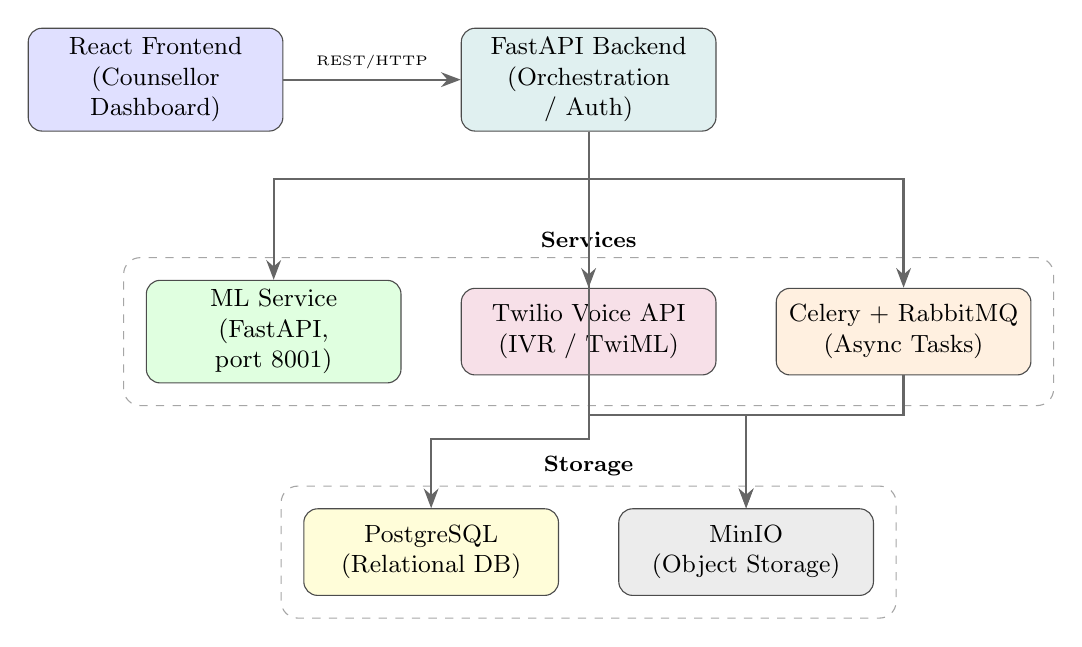
\begin{tikzpicture}[
  svc/.style={rectangle, rounded corners=5pt, draw=black!70, minimum height=1.1cm,
              text width=3.0cm, align=center, font=\small},
  dbarrow/.style={-{Stealth[length=2.5mm]}, thick, draw=black!60},
  grp/.style={draw=black!35, dashed, rounded corners=6pt, inner sep=8pt},
  lbl/.style={font=\footnotesize\bfseries}
]
  % ---- Frontend ----
  \node[svc, fill=blue!12] (fe) at (0,0) {React Frontend\\(Counsellor Dashboard)};

  % ---- Backend ----
  \node[svc, fill=teal!12] (be) at (5.5,0) {FastAPI Backend\\(Orchestration / Auth)};

  % ---- Services row ----
  \node[svc, fill=green!12]  (ml)   at (1.5,-3.2) {ML Service\\(FastAPI, port 8001)};
  \node[svc, fill=purple!12] (twil) at (5.5,-3.2) {Twilio Voice API\\(IVR / TwiML)};
  \node[svc, fill=orange!12] (cely) at (9.5,-3.2) {Celery + RabbitMQ\\(Async Tasks)};

  % ---- Storage row ----
  \node[svc, fill=yellow!15] (pg)    at (3.5,-6.0) {PostgreSQL\\(Relational DB)};
  \node[svc, fill=gray!15]   (minio) at (7.5,-6.0) {MinIO\\(Object Storage)};

  % ---- Arrows ----
  \draw[dbarrow] (fe.east)  -- node[above,font=\tiny]{REST/HTTP} (be.west);

  \draw[dbarrow] (be.south) -- ++(0,-0.6) -| (ml.north);
  \draw[dbarrow] (be.south) -- ++(0,-0.6) -- (twil.north);
  \draw[dbarrow] (be.south) -- ++(0,-0.6) -| (cely.north);

  \draw[dbarrow] (be.south)  -- ++(0,-3.9) -| (pg.north);
  \draw[dbarrow] (cely.south)-- ++(0,-0.5) -| (minio.north);
  \draw[dbarrow] (twil.south)-- ++(0,-0.5) -| (minio.north);

  % ---- Group labels ----
  \begin{scope}[on background layer]
    \node[grp, fit=(ml)(twil)(cely), label={[lbl]above:Services}] {};
    \node[grp, fit=(pg)(minio),       label={[lbl]above:Storage}] {};
  \end{scope}
\end{tikzpicture}}
\caption{High-level microservices architecture of the proposed mHealth system. The React frontend communicates with the FastAPI backend, which orchestrates the ML service, Twilio IVR, and Celery task queue. Audio recordings are persisted in MinIO; metadata in PostgreSQL.}
\label{fig:system_arch}
\end{figure}

\begin{table}[h]
\centering
\caption{Technology stack for the proposed mHealth system.}
\label{tab:tech_stack}
\begin{tabular}{@{}lll@{}}
\toprule
\textbf{Component} & \textbf{Technology} & \textbf{Role} \\
\midrule
Frontend           & React (TypeScript), Vite, MUI & Counsellor dashboard \\
Backend API        & FastAPI (Python)               & Orchestration, routing, auth \\
ML Service         & FastAPI (Python)               & Depression inference \\
IVR / Call Service & Twilio Voice API + FastAPI     & Outbound calls, TwiML \\
Task Queue         & Celery + RabbitMQ             & Async archival and ML inference \\
Database           & PostgreSQL + SQLAlchemy        & Persistent storage \\
Object Storage     & MinIO                         & Audio recording archival \\
Migrations         & Alembic                       & Schema versioning \\
Authentication     & JWT                           & Admin access control \\
\bottomrule
\end{tabular}
\end{table}

%-------------------------------------------------------------
\section{Component Descriptions}
%-------------------------------------------------------------

\subsection{Frontend: Counsellor Dashboard}

The frontend is a React single-page application (SPA) built with TypeScript, Vite, and Material UI (MUI). It communicates with the backend exclusively via RESTful HTTP and provides a unified interface for all counsellor-facing operations.

\subsubsection{Authentication}

Access to the dashboard is controlled by JWT-based authentication. Figure~\ref{fig:ui_login} shows the login screen, which supports both direct email/password login and institute single sign-on via INAS (Institute Authentication Services).

\begin{figure}[h]
    \centering
    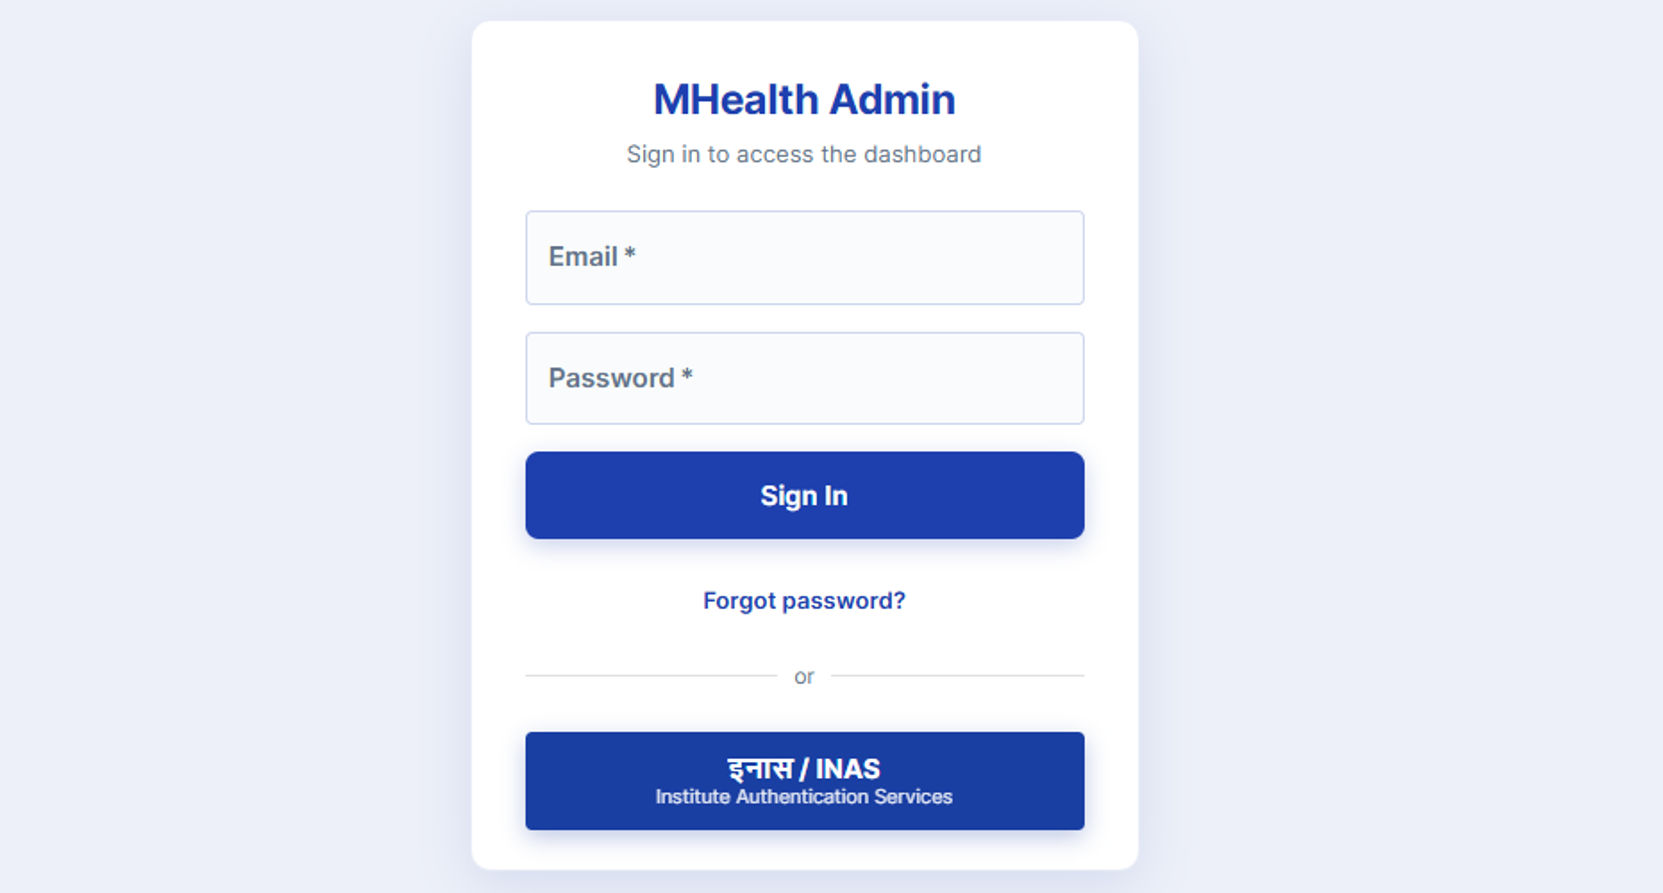
\includegraphics[width=0.75\textwidth]{Pictures/ui_login_cropped2.png}
    \caption{MHealth Admin login page. Supports email/password authentication and IITGN Institute Authentication Services (INAS) single sign-on.}
    \label{fig:ui_login}
\end{figure}

\subsubsection{Landing Page and Navigation}

After login, the counsellor is presented with the platform's landing page (Figure~\ref{fig:ui_about}), which provides navigation to three operational modules: Twilio Call Management, Call Status Dashboard, and Admin Dashboard.

\begin{figure}[h]
    \centering
    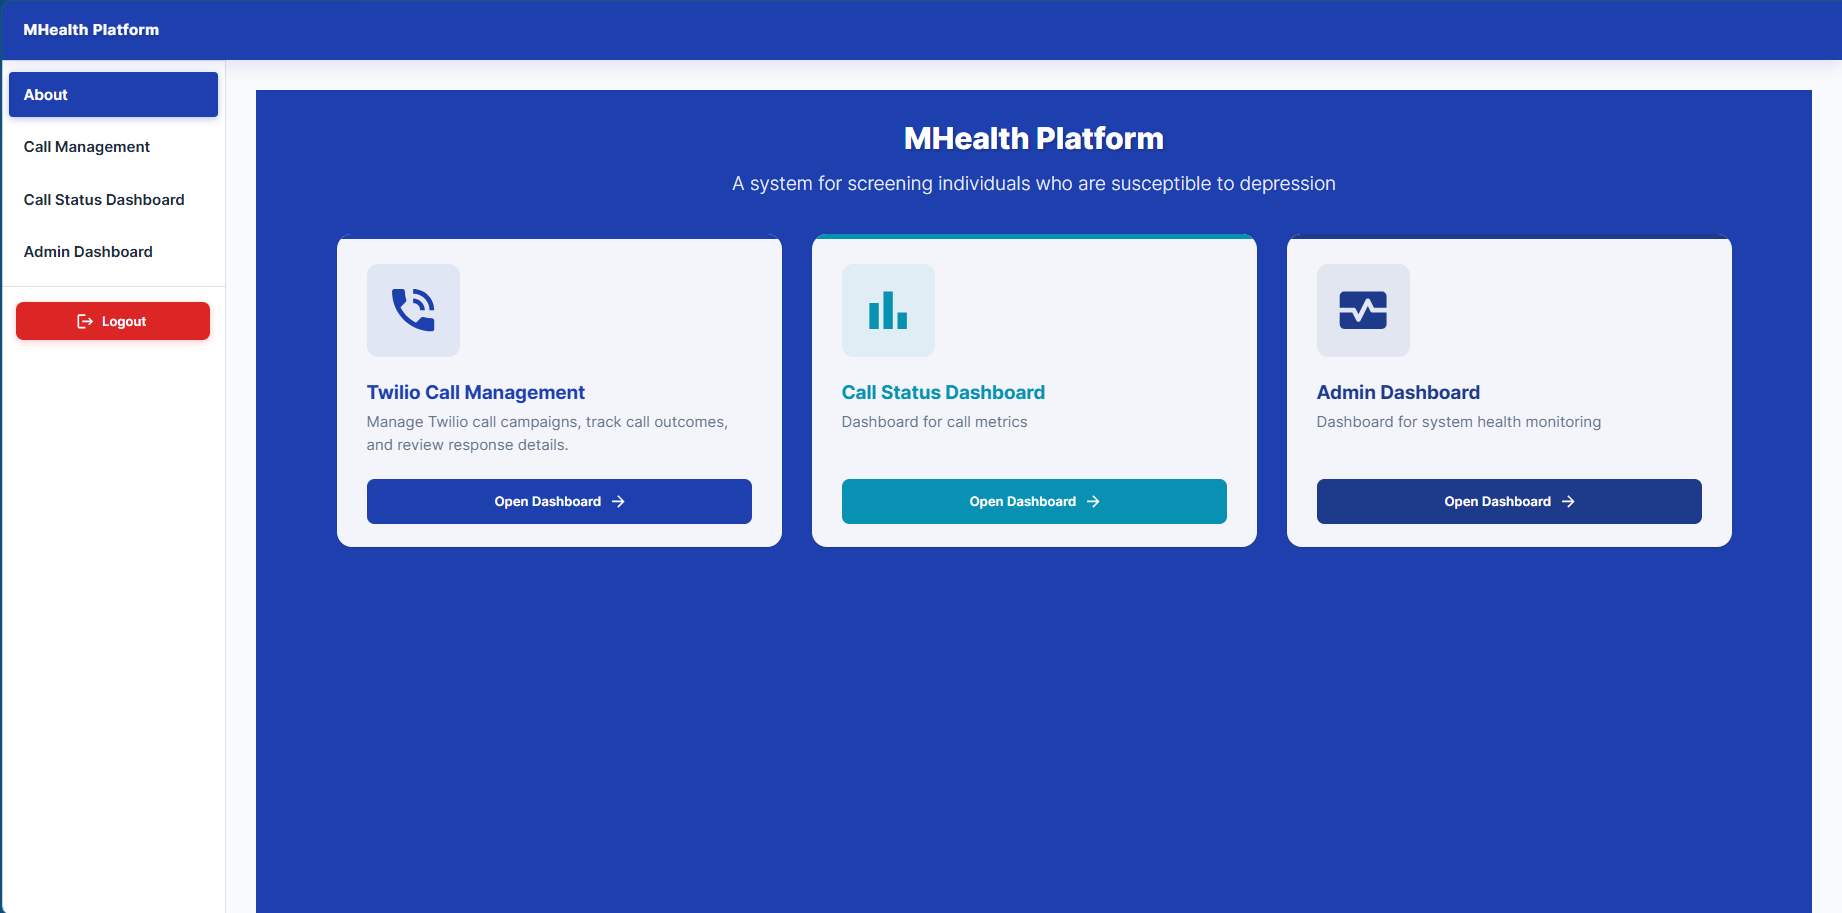
\includegraphics[width=\textwidth]{Pictures/ui_about.png}
    \caption{MHealth Platform landing page showing the three primary modules available to the counsellor after authentication.}
    \label{fig:ui_about}
\end{figure}

\subsubsection{Call Management Page}

The Call Management page (Figure~\ref{fig:ui_call_mgmt}) is the primary operational interface. It allows counsellors to:
\begin{itemize}
    \item Add individual recipients or import a list via CSV/XLSX.
    \item Select recipients and initiate Twilio calls immediately.
    \item View call history for each recipient: scheduled time, answer time, end time, overall duration, total response duration, and questions answered.
    \item Review the ML-predicted depression risk probability (e.g., \texttt{Risk Probability: 0.485} as shown in Figure~\ref{fig:ui_call_mgmt}).
    \item Play back the audio recording for each individual question response directly in the browser.
\end{itemize}

\begin{figure}[h]
    \centering
    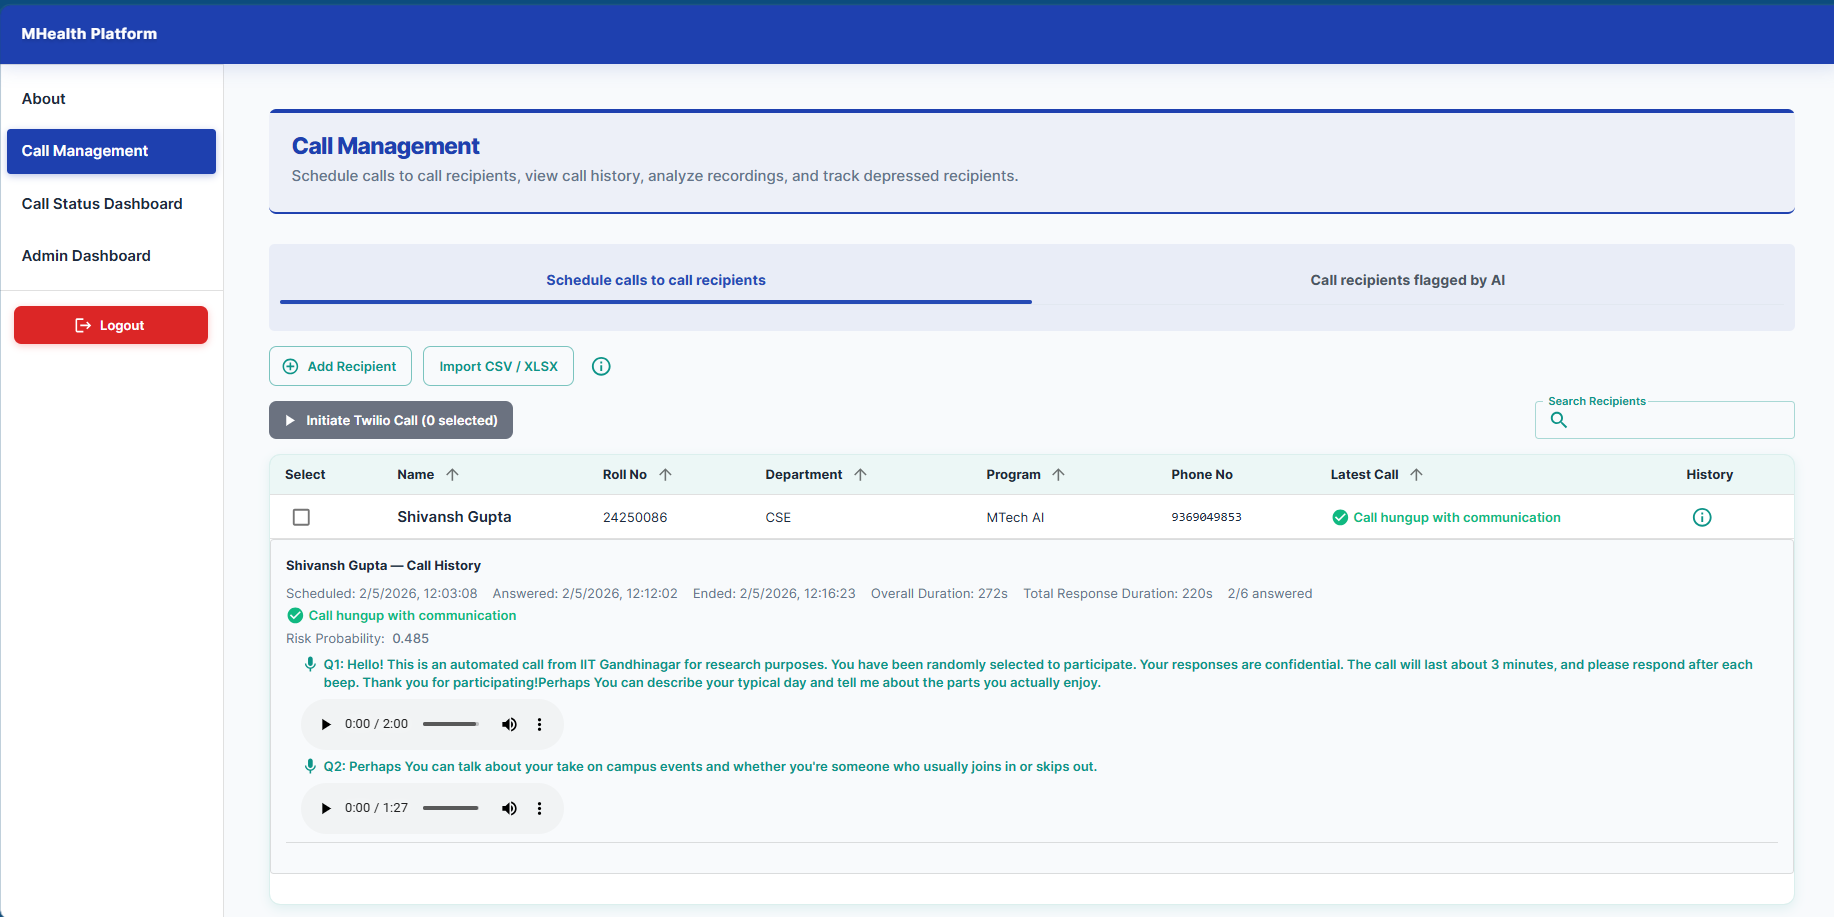
\includegraphics[width=\textwidth]{Pictures/ui_call_management.png}
    \caption{Call Management page showing a completed call for a recipient (roll no.\ 24250086). The call history panel displays the scheduled and answer times, duration, risk probability (0.485), and in-browser audio playback for each of the 6 question responses.}
    \label{fig:ui_call_mgmt}
\end{figure}

\subsubsection{AI-Flagged Recipients Tab}

Within the Call Management page, the ``Call recipients flagged by AI'' tab (Figure~\ref{fig:ui_flagged}) presents a dedicated table of students whose risk probability exceeds 0.5. This implements the human-in-the-loop design goal: the counsellor reviews this list and decides which individuals warrant follow-up. The table includes name, roll number, department, program, call timestamp, and analysis score. An export function allows the list to be downloaded for offline review.

\begin{figure}[h]
    \centering
    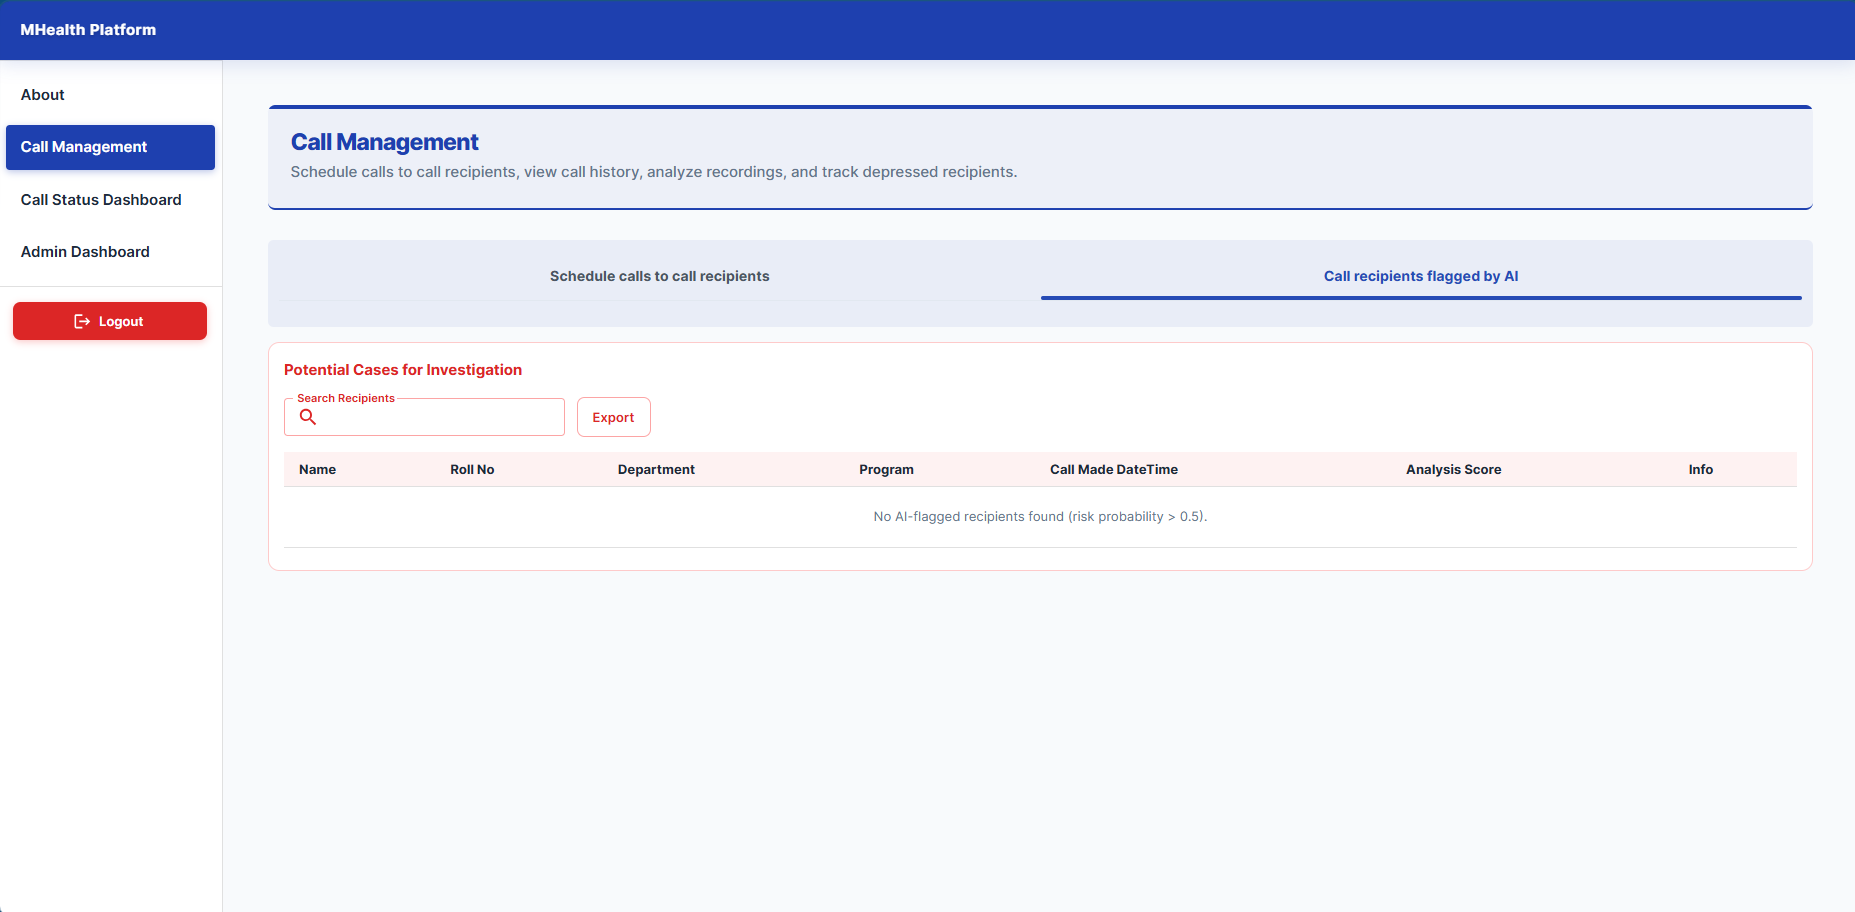
\includegraphics[width=\textwidth]{Pictures/ui_ai_flagged.png}
    \caption{``Call recipients flagged by AI'' tab showing potential cases for investigation (risk probability $> 0.5$). The counsellor reviews this list and independently decides on clinical follow-up — no automated action is taken.}
    \label{fig:ui_flagged}
\end{figure}

\subsubsection{Call Status Dashboard}

The Call Status Dashboard (Figure~\ref{fig:ui_status}) provides a real-time aggregate overview of all screening activity. It displays:
\begin{itemize}
    \item \textbf{Recipient Metrics}: Total call recipients, total predicted as depressed by the ML model, and predictions in the last 24 hours.
    \item \textbf{Call Metrics}: Total calls made and calls in the last 24 hours.
    \item \textbf{Calls by Status}: Breakdown across all call states — Scheduled, Initiated, In Progress, Not Picked, Hungup with Communication, Hungup with Short Communication, and Failed.
\end{itemize}

\begin{figure}[h]
    \centering
    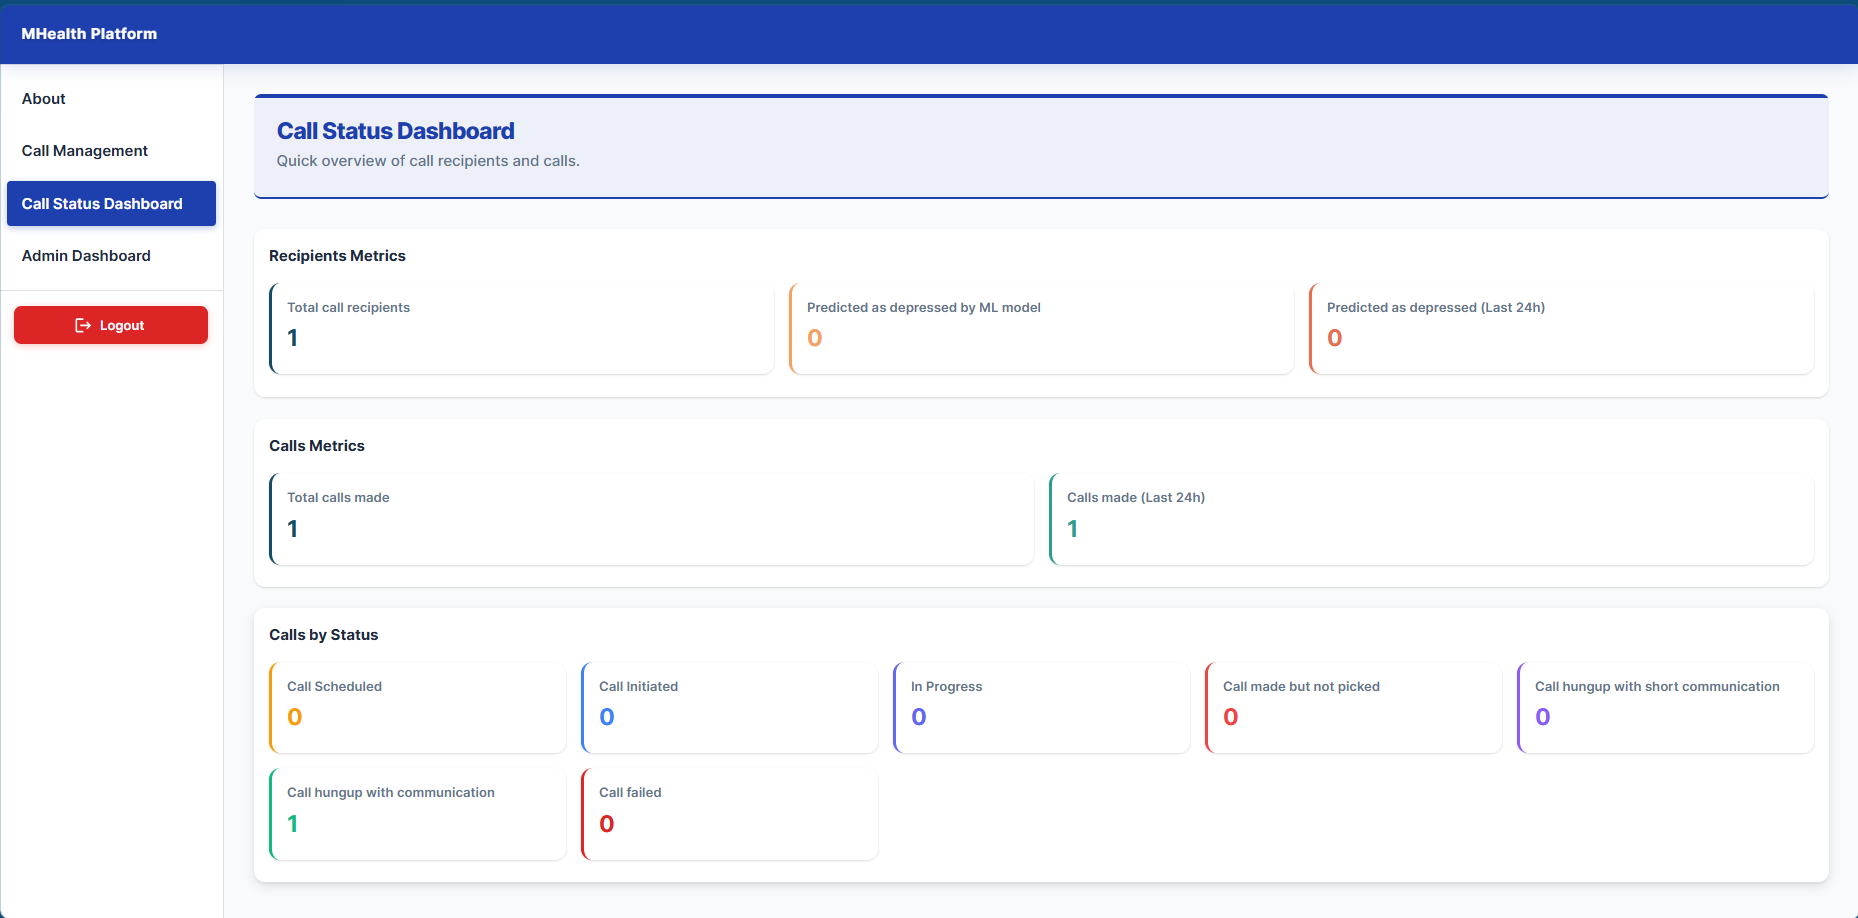
\includegraphics[width=\textwidth]{Pictures/ui_call_status.png}
    \caption{Call Status Dashboard showing recipient metrics (total recipients, ML depression predictions), call volume metrics, and a breakdown of all call outcomes by status category.}
    \label{fig:ui_status}
\end{figure}

\subsubsection{Admin Dashboard}

The Admin Dashboard (Figure~\ref{fig:ui_admin}) provides system health monitoring for the operator. It shows real-time status of all four infrastructure components — API, MinIO, Twilio SID, and Webhooks — with green checkmarks indicating operational status. It also displays the configuration overview (MinIO endpoint, bucket name, Twilio account SID, app host) and the exact webhook URLs registered with Twilio (\texttt{/voice/answer}, \texttt{/voice/status}, \texttt{/twilio}).

\begin{figure}[h]
    \centering
    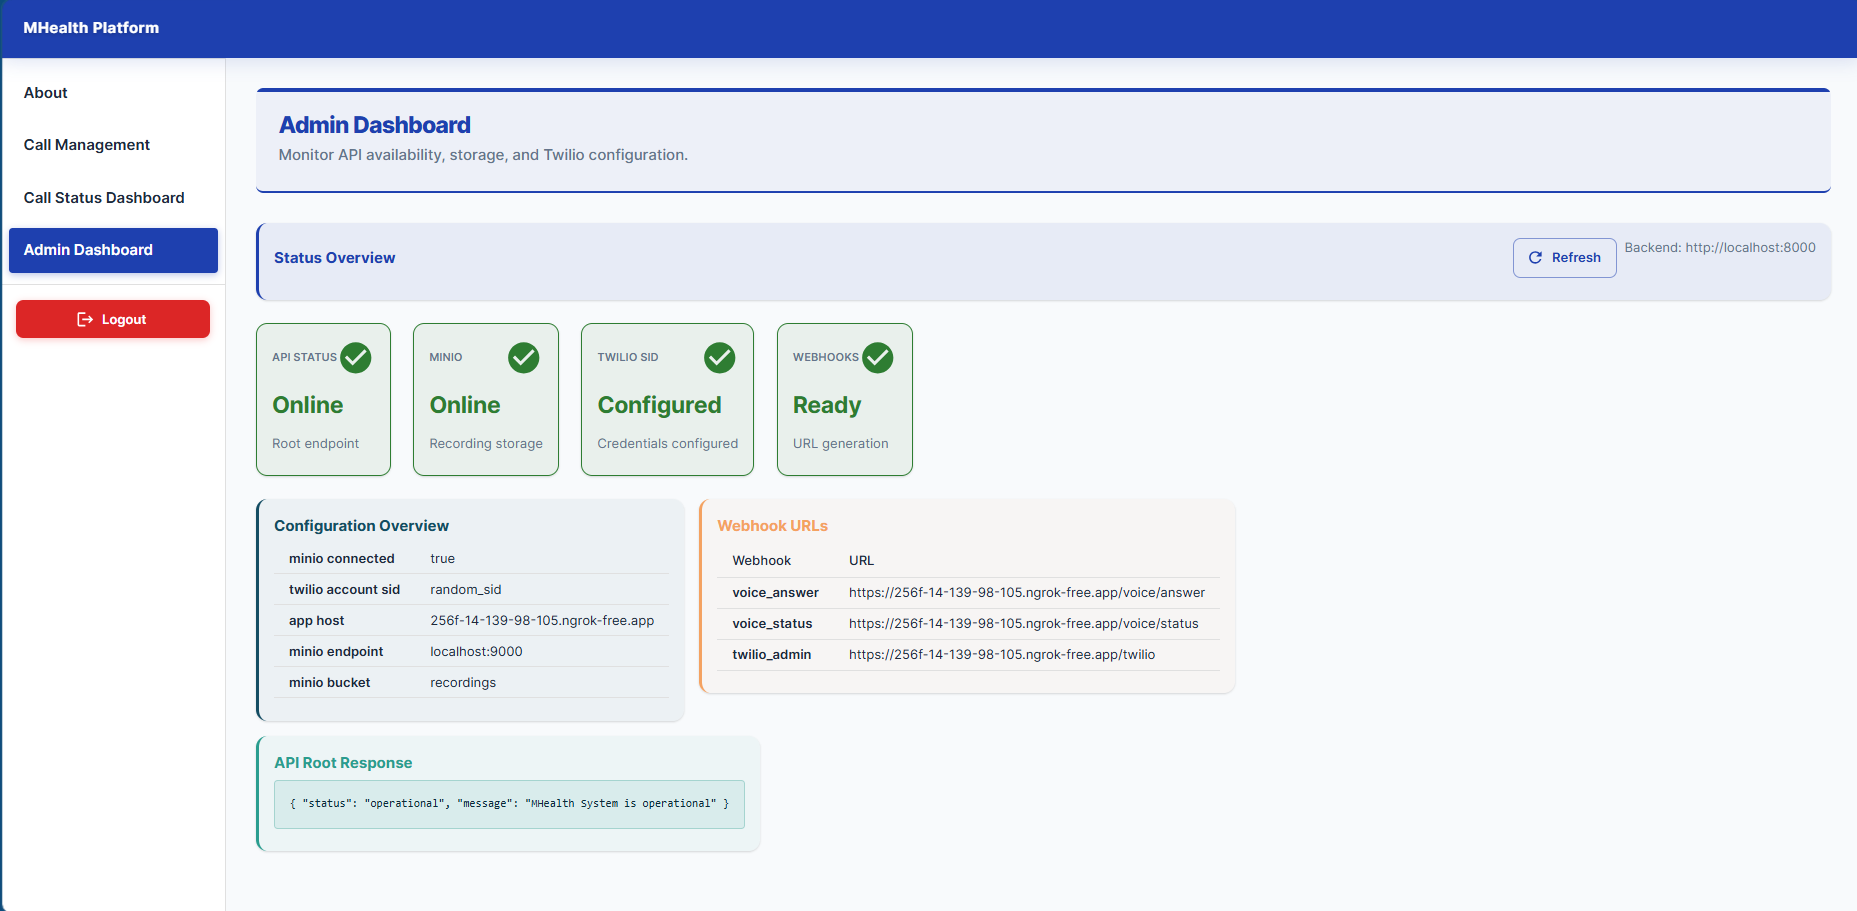
\includegraphics[width=\textwidth]{Pictures/ui_admin.png}
    \caption{Admin Dashboard showing live system health: API online, MinIO connected, Twilio SID configured, and webhooks ready. The configuration panel and active webhook URLs are displayed for operator verification.}
    \label{fig:ui_admin}
\end{figure}

\subsection{Backend API}

The main backend is a FastAPI application serving as the central orchestration layer. It exposes the following router groups:
\begin{itemize}
    \item \textbf{Auth routes} (\texttt{/auth}): Login, password reset.
    \item \textbf{ML routes} (\texttt{/api/ml}): Proxy to the ML service.
    \item \textbf{Database routes} (\texttt{/api/db}): CRUD on the main database.
    \item \textbf{Call monitoring routes} (\texttt{/api/calls}): Aggregated statistics.
    \item \textbf{Target monitoring routes} (\texttt{/api/targets}): Target-level summaries.
    \item \textbf{Counsellor routes} (\texttt{/api/counsellor}): Flagging and clinical review.
    \item \textbf{Twilio admin routes} (\texttt{/twilio}): Call initiation, history.
    \item \textbf{Twilio webhook routes} (\texttt{/voice/answer}, \texttt{/voice/respond/\{q\}}, \texttt{/voice/status}): Twilio callbacks.
\end{itemize}

\subsection{IVR Service: Twilio Voice Call Flow}

The IVR service implements the outbound call workflow using the Twilio Voice API.

\subsubsection{Call Flow}

\begin{enumerate}
    \item A counsellor triggers call initiation via the Call Management page; the backend creates a \texttt{TwilioCalls} record and queues \texttt{initiate\_twilio\_call\_task}.
    \item The Celery worker places the call using \texttt{twilio.rest.\allowbreak Client.calls.\allowbreak create()}, specifying webhook URLs for call answer and status events.
    \item When the student answers, Twilio POSTs to \texttt{/voice/answer}; the server returns TwiML for Question~0.
    \item For each question, Twilio plays the TTS prompt (Amazon Polly, \texttt{Raveena} voice, \texttt{en-IN} locale) and records the student's response via \texttt{<Record>}.
    \item After recording, Twilio POSTs to \texttt{/voice/respond/\{q\}}; the server stores the response and returns TwiML for the next question.
    \item The call ends after all 6 prompts or when total response duration reaches 180 seconds.
    \item Upon completion, two Celery tasks are queued: audio archival and ML inference.
\end{enumerate}

\subsubsection{Call Prompts}

The six open-ended prompts are designed to elicit natural, conversational speech, framed around everyday positive topics to reduce anxiety:
\begin{enumerate}
    \item Perhaps you can describe your typical day and tell me about the parts you actually enjoy.
    \item Perhaps you can talk about your take on campus events and whether you're someone who usually joins in or skips out.
    \item Describe your favourite college memory.
    \item Talk about how you and friends spend time outside class.
    \item Mention clubs or activities you are part of and what you enjoy.
    \item Share anything else on your mind about your college experience.
\end{enumerate}

All incoming Twilio webhook requests are validated against the \texttt{X-Twilio-Signature} header to prevent spoofed requests.

\subsection{ML Service}

The ML service is a dedicated FastAPI application running on port 8001. Key endpoints:
\begin{itemize}
    \item \texttt{POST /api/ml/depression}: Single-call depression prediction from audio bytes.
    \item \texttt{POST /api/ml/depression-batch}: Batch prediction for multiple files.
    \item \texttt{POST /warmup}: Pre-loads the model before traffic begins.
    \item \texttt{GET /health}: Health check with model load status.
\end{itemize}

The service uses lazy initialisation: the Random Forest model is loaded on the first prediction request, allowing the container to pass health checks before the model is ready.

\subsection{Asynchronous Task Queue: Celery and RabbitMQ}

Long-running operations are handled asynchronously by Celery workers via RabbitMQ:

\begin{table}[h]
\centering
\caption{Celery tasks in the system.}
\label{tab:celery_tasks}
\resizebox{\textwidth}{!}{%
\begin{tabular}{@{}p{6.2cm}p{8.5cm}@{}}
\toprule
\textbf{Task} & \textbf{Description} \\
\midrule
\texttt{initiate\_twilio\_call\_task}          & Places one outbound Twilio call; retries up to 3 times \\[4pt]
\texttt{archive\_call\_recordings\_task}       & Fan-out: queues one archival task per voice response \\[4pt]
\texttt{archive\_response\_recording\_task}    & Downloads one recording, uploads to MinIO, extracts duration via \texttt{ffprobe} \\[4pt]
\texttt{analyze\_call\_depression\_risk\_task} & Concatenates responses, invokes ML service, stores prediction \\[4pt]
\texttt{initiate\_calls\_for\_all\_targets}    & Defined in codebase but not active; calls are initiated manually by the counsellor via the dashboard \\
\bottomrule
\end{tabular}}
\end{table}

\subsection{Database: PostgreSQL with SQLAlchemy}

The PostgreSQL schema supports the complete counselling workflow:

\begin{table}[h]
\centering
\caption{Key database tables.}
\label{tab:db_schema}
\resizebox{\textwidth}{!}{%
\begin{tabular}{@{}p{4.8cm}p{9.5cm}@{}}
\toprule
\textbf{Table} & \textbf{Description} \\
\midrule
\texttt{TwilioTargets}           & Students enrolled in the screening programme \\
\texttt{TwilioCalls}             & Call records with depression prediction fields: risk flag, probability, level, confidence, timestamp \\
\texttt{TwilioResponses}         & Per-question responses: Twilio URL, MinIO URL, duration, question text \\
\texttt{Admins}                  & Counsellor accounts (email, hashed password) \\
\texttt{FlaggedTargets}          & Students flagged for counsellor follow-up \\
\texttt{Error\_Logs}             & System error entries \\
\texttt{Password\_Reset\_Tokens} & Time-limited tokens for password reset \\
\bottomrule
\end{tabular}}
\end{table}

\subsection{Object Storage: MinIO}

Twilio recording URLs are temporary and require authentication. To ensure long-term availability and institutional data ownership, recordings are archived to a self-hosted MinIO instance at the path:
\begin{verbatim}
twilio/{YYYY}/{MM}/{DD}/{call_sid}/{recording_filename}
\end{verbatim}

Playback is provided via presigned URLs with a 1-hour expiry. If MinIO is unavailable, the system falls back to Twilio-authenticated URLs, ensuring the ML pipeline is not blocked.

%-------------------------------------------------------------
\section{Data Flow Summary}
%-------------------------------------------------------------

The end-to-end data flow is as follows:
\begin{enumerate}
    \item Counsellor adds recipients and initiates calls from the Call Management page $\rightarrow$ DB record created $\rightarrow$ Celery queues call task.
    \item Twilio calls student $\rightarrow$ student answers $\rightarrow$ TwiML serves Question~0.
    \item Student responds (recorded) $\rightarrow$ Twilio POSTs to \texttt{/voice/respond/0}.
    \item Response saved $\rightarrow$ next prompt served; repeated for all 6 prompts.
    \item After Question~5 or 3-minute limit: call ends $\rightarrow$ archival and ML tasks queued.
    \item Archival task: recordings downloaded $\rightarrow$ uploaded to MinIO.
    \item ML task: audio concatenated $\rightarrow$ sent to ML service $\rightarrow$ prediction stored in \texttt{TwilioCalls}.
    \item Counsellor reviews Call Management page: risk probability visible, audio playback available per question (Figure~\ref{fig:ui_call_mgmt}).
    \item Students with risk probability $>$ 0.5 appear in the AI-flagged tab (Figure~\ref{fig:ui_flagged}); counsellor decides on follow-up.
\end{enumerate}

%-------------------------------------------------------------
\section{Deployment}
%-------------------------------------------------------------

The system is containerised with Docker, with separate containers for the backend, ML service, frontend, PostgreSQL, RabbitMQ, and MinIO. HTTPS is enforced at the application boundary, ensuring all Twilio webhook traffic and counsellor API calls are encrypted in transit. The Admin Dashboard (Figure~\ref{fig:ui_admin}) allows operators to verify at a glance that all infrastructure components are healthy before commencing a call campaign.

%-------------------------------------------------------------
\section{Summary}
%-------------------------------------------------------------

The proposed mHealth system is a microservices-based platform designed around seven principles: scalability, interpretability, human-in-the-loop oversight, privacy, non-intrusiveness, workflow integration, and continual improvement. Its implementation integrates Twilio IVR for automated voice collection, Celery for asynchronous processing, TSFEL-based ML inference for depression risk prediction, MinIO for secure audio storage, PostgreSQL for structured data management, and a React dashboard for counsellor interaction. The six dashboard screenshots presented in this chapter demonstrate a fully operational system deployed and tested at IIT Gandhinagar.

\chapter{Pilot Trial}
\label{Chapter5}

This chapter presents the pilot trial conducted to evaluate the proposed mHealth system with real users. The trial involved 10 Master's degree students at IIT Gandhinagar and collected spoken audio responses to a structured set of conversational prompts. The collected audio was processed through the complete ML pipeline described in Chapter~\ref{Chapter3} to produce depression risk predictions. Both quantitative analysis (prediction results, response durations, segment counts) and qualitative observations are reported.

%=============================================================
\section{Study Setup}
%=============================================================

\subsection{Participants}

Ten Master's degree students from IIT Gandhinagar participated in the pilot trial. All participants were enrolled in postgraduate programmes and voluntarily agreed to take part. Participation was anonymous; each participant is identified by a pseudonym (User1–User10) throughout this chapter. Informed consent was obtained from all participants prior to data collection.

\subsection{Data Collection Instrument}

Each participant was asked to respond verbally to a structured set of 10 open-ended conversational prompts. The prompts were intentionally designed to be non-clinical and conversational, covering everyday topics related to mood, habits, goals, and aspirations. The prompts are listed in Table~\ref{tab:questionnaire}.

\begin{table}[h]
\centering
\caption{Conversational prompts used for audio data collection in the pilot trial.}
\label{tab:questionnaire}
\begin{tabular}{@{}cp{10.5cm}@{}}
\toprule
\textbf{P\#} & \textbf{Prompt} \\
\midrule
P1  & How is your day going so far? \\
P2  & What are your plans for today? \\
P3  & How are you feeling right now? \\
P4  & What are some of your daily habits? \\
P5  & What changes would you like to see in yourself a year from now? \\
P6  & What do you enjoy doing in your free time? \\
P7  & What motivates you to keep going every day? \\
P8  & How do you usually start your mornings? \\
P9  & What is something new you have learned recently? \\
P10 & Where do you see yourself after graduating from IIT Gandhinagar? \\
\bottomrule
\end{tabular}
\end{table}

\subsection{Audio Recording Procedure}

Responses were recorded individually for each prompt as separate audio files in Opus format at 16\,kHz. The complete set of recordings for each participant was stored under a per-user directory inside \texttt{questionnaire\_audio\_data.zip}.

Prior to ML inference, all 10 response files per user were loaded with \texttt{librosa} (sr\,=\,16\,000\,Hz, mono), resampled to a common sample rate, and concatenated into a single continuous audio stream using \texttt{numpy.concatenate()}, following the same pipeline as the production system (Section~\ref{sec:pipeline_detail}).

%=============================================================
\section{Response Duration Analysis}
%=============================================================

Table~\ref{tab:durations} reports the duration of each individual response and the total cumulative speech duration per participant. These figures reflect the amount of acoustic information available to the ML model for each user.

\begin{table}[h]
\centering
\caption{Per-prompt response duration (seconds) and total duration per participant.}
\label{tab:durations}
\resizebox{\textwidth}{!}{%
\begin{tabular}{@{}lrrrrrrrrrrrr@{}}
\toprule
\textbf{User} & \textbf{P1} & \textbf{P2} & \textbf{P3} & \textbf{P4} & \textbf{P5} & \textbf{P6} & \textbf{P7} & \textbf{P8} & \textbf{P9} & \textbf{P10} & \textbf{Total (s)} & \textbf{Segs} \\
\midrule
User1  & 5.5  & 5.3  & 3.7  & 5.2  & 4.4  & 4.9  & 5.2  & 3.9  & 4.2  & 5.9  & 48.2  & 7  \\
User2  & 6.4  & 8.0  & 5.3  & 4.8  & 3.6  & 6.0  & 4.3  & 8.0  & 8.8  & 5.8  & 61.0  & 8  \\
User3  & 5.5  & 9.8  & 11.0 & 17.8 & 5.9  & 9.2  & 19.4 & 8.7  & 11.2 & 8.5  & 106.9 & 14 \\
User4  & 2.5  & 5.3  & 3.3  & 16.8 & 4.8  & 3.3  & 1.8  & 8.3  & 12.9 & 1.3  & 60.2  & 8  \\
User5  & 7.0  & 14.2 & 8.4  & 12.0 & 9.2  & 8.7  & 13.9 & 11.8 & 13.2 & 12.2 & 110.5 & 14 \\
User6  & 10.8 & 11.6 & 3.7  & 17.5 & 24.8 & 21.5 & 24.9 & 9.8  & 12.6 & 30.6 & 167.8 & 21 \\
User7  & 10.4 & 9.0  & 10.2 & 19.6 & 14.2 & 16.7 & 13.7 & 13.6 & 17.7 & 15.8 & 140.8 & 18 \\
User8  & 10.1 & 9.9  & 7.0  & 15.3 & 10.7 & 14.9 & 11.6 & 14.3 & 10.0 & 6.0  & 109.9 & 14 \\
User9  & 5.3  & 5.2  & 2.9  & 6.8  & 3.0  & 4.2  & 3.6  & 13.7 & 13.5 & 24.1 & 82.3  & 11 \\
User10 & 8.8  & 8.7  & 2.9  & 6.2  & 6.9  & 8.9  & 9.6  & 9.8  & 12.0 & 13.0 & 86.8  & 11 \\
\midrule
\textbf{Mean} & 7.2 & 8.7 & 5.8 & 12.2 & 8.8 & 9.8 & 10.8 & 10.2 & 11.6 & 12.3 & 97.4 & 12.6 \\
\bottomrule
\end{tabular}}
\end{table}

\noindent\textbf{Observations from duration analysis:}
\begin{itemize}
    \item Total response durations ranged from 48.2\,s (User1, 7 segments) to 167.8\,s (User6, 21 segments), reflecting substantial individual variation in verbosity.
    \item Prompts P9 and P10 (future goals and post-graduation plans) elicited the longest average responses (11.6\,s and 12.3\,s respectively), likely because they invite more elaborate and forward-looking reflection.
    \item Prompt P3 (``How are you feeling right now?'') produced the shortest average responses (5.8\,s), consistent with the tendency to give brief answers to direct emotional questions.
    \item The segment count (final column) is derived by dividing the total concatenated audio duration by the 7-second segment window, which determines how many independent feature vectors are fed to the Random Forest.
\end{itemize}

%=============================================================
\section{Quantitative Analysis: Depression Risk Predictions}
%=============================================================

Table~\ref{tab:pilot_results} presents the full depression risk prediction results produced by the ML pipeline for all 10 participants.

\begin{table}[h]
\centering
\caption{Depression risk prediction results for all 10 pilot participants.}
\label{tab:pilot_results}
\resizebox{\textwidth}{!}{%
\begin{tabular}{@{}lcccccr@{}}
\toprule
\textbf{User} & \textbf{Risk} & \textbf{Probability} & \textbf{Level} & \textbf{Confidence} & \textbf{Segments} & \textbf{Total (s)} \\
\midrule
User1  & 1 & 0.5356 & \textbf{High} & 0.5356 & 7  & 48.2  \\
User2  & 0 & 0.3916 & Low           & 0.6084 & 8  & 61.0  \\
User3  & 0 & 0.4209 & Low           & 0.5791 & 14 & 106.9 \\
User4  & 0 & 0.3485 & Low           & 0.6515 & 8  & 60.2  \\
User5  & 0 & 0.4464 & Low           & 0.5536 & 14 & 110.5 \\
User6  & 0 & 0.2953 & Low           & 0.7047 & 21 & 167.8 \\
User7  & 0 & 0.4353 & Low           & 0.5647 & 18 & 140.8 \\
User8  & 1 & 0.5922 & \textbf{High} & 0.5922 & 14 & 109.9 \\
User9  & 0 & 0.4169 & Low           & 0.5831 & 11 & 82.3  \\
User10 & 0 & 0.3674 & Low           & 0.6326 & 11 & 86.8  \\
\midrule
\multicolumn{7}{@{}l}{\textit{Summary: 2/10 predicted High risk \quad Average probability: 0.4250}} \\
\bottomrule
\end{tabular}}
\end{table}

\subsection{Key Quantitative Findings}

\begin{itemize}
    \item \textbf{2 out of 10 participants (20\%) were predicted as High risk} (depression\_risk\,=\,1) by the model — User1 (probability: 0.5356) and User8 (probability: 0.5922).
    \item \textbf{Average risk probability across all participants: 0.4250}, which is below the 0.5 decision threshold, indicating that the majority of participants were classified as Low risk.
    \item \textbf{User8 had the highest risk probability (0.5922)} and the highest confidence in the High-risk direction, with the longest sustained speech patterns across multiple responses.
    \item \textbf{User6 had the lowest risk probability (0.2953)} and the highest confidence (0.7047), suggesting acoustically clear low-risk features; this participant also had the longest total recording duration (167.8\,s, 21 segments).
    \item \textbf{Borderline cases}: User3 (0.4209), User5 (0.4464), and User7 (0.4353) all had probabilities in the range 0.42–0.45 — close to the threshold, warranting counsellor attention even though classified as Low risk.
    \item \textbf{Confidence scores} for Low-risk predictions ranged from 0.5536 (User5) to 0.7047 (User6), reflecting varying degrees of model certainty. Lower confidence scores in the Low-risk group identify participants worth monitoring.
\end{itemize}


%=============================================================
\section{Qualitative Analysis}
%=============================================================

\subsection{Participant Feedback}

Following the recording session, participants were asked informally about their experience with the prompt format. General themes from participant feedback included:

\begin{itemize}
    \item \textbf{Naturalness of prompts}: Most participants found the open-ended conversational format comfortable and non-threatening, consistent with the design goal of non-intrusiveness (DG5).
    \item \textbf{Prompt depth}: Prompts about future goals (P10) and motivation (P7) elicited the most detailed and emotionally expressive responses, as evidenced by their longer average durations.
    \item \textbf{Privacy concerns}: Several participants expressed comfort with audio data being handled within the institute's own infrastructure rather than sent to third-party cloud services, validating the MinIO self-hosting design choice (DG4).
    \item \textbf{Awareness of AI screening}: When informed that their audio would be processed by a machine learning model, participants generally expressed acceptance, provided that a counsellor would review and act on any flagged cases — directly corroborating the necessity of DG3 (Human-in-the-Loop).
\end{itemize}

\subsection{Observations on System Behaviour}

\begin{itemize}
    \item The \texttt{run\_predictions.py} script successfully processed all 10 users without errors, confirming end-to-end pipeline robustness.
    \item The number of 7-second segments per user scaled naturally with total response duration, ranging from 7 segments (User1, 48.2\,s) to 21 segments (User6, 167.8\,s).
    \item The mean probability of 0.4250 across all participants is below the 0.5 threshold, which is expected in a healthy student sample where most participants do not exhibit strong depressive acoustic patterns.
    \item The two flagged participants (User1 and User8) represent 20\% of the cohort, which is slightly below the clinical prevalence reported in similar university populations~\cite{BlackDeer2023}, suggesting the model's threshold may be appropriately calibrated for this setting.
\end{itemize}

%=============================================================
\section{Limitations}
%=============================================================

\begin{itemize}
    \item \textbf{No ground-truth labels}: Participants were not assessed using a validated clinical instrument (e.g., PHQ-9) during this pilot, so it is not possible to compute sensitivity, specificity, or classification accuracy. This is a known limitation of the pilot phase and is addressed in the future work plan (Chapter~\ref{Chapter7}).
    \item \textbf{Small sample size}: With only 10 participants, statistical conclusions cannot be drawn. This trial serves as a feasibility demonstration rather than a clinical evaluation.
    \item \textbf{Controlled recording environment}: Audio was recorded in a controlled setting rather than collected via the Twilio IVR system used in production, introducing a potential domain gap relative to real deployment conditions (telephone-quality audio, background noise).
    \item \textbf{Self-selection bias}: Participants who volunteered may differ systematically from the broader student population.
\end{itemize}

%=============================================================
\section{Summary}
%=============================================================

The pilot trial collected audio responses from 10 Master's degree students at IIT Gandhinagar across a 10-prompt conversational session. The ML pipeline processed a total of 97.4 seconds of speech per participant on average, segmented into 12.6 seven-second windows. The model predicted 2 out of 10 participants as High risk (depression probability $>$ 0.5), with an average cross-participant probability of 0.4250. User8 received the highest risk probability (0.5922) and User6 the lowest (0.2953). Three participants in the borderline range (0.42–0.45) were identified for potential counsellor monitoring. The trial confirms the technical feasibility of the end-to-end pipeline and provides an initial indication of the system's behaviour on a real student cohort.

\chapter{Conclusion}
\label{Chapter6}

This thesis addressed the problem of automated, interpretable, and scalable depression detection from speech in a university setting. The work spanned two interconnected technical threads — Speech Emotion Recognition (SER) preliminary experiments and a full depression detection pipeline on the DAIC-WOZ corpus — implemented within a complete mHealth system for institutional deployment.

\section{Summary of Contributions}

\textbf{SER Preliminary Experiments.} A series of speech emotion recognition experiments explored custom feature engineering (pause-histogram features and mel-spectrogram features) combined with multiple deep neural network architectures: a 2D CNN with Squeeze-and-Excitation residual blocks, a 1D CNN + LSTM model, and a 2D CNN + BiGRU model. These were evaluated on RAVDESS, CREMA-D, EMO-DB, TESS, IESC. The experiments informed two key design decisions for the depression pipeline: the value of aggregating frame-level features using descriptive statistics, and the importance of combining spectral and temporal features.

\textbf{ML Processing Pipeline.} A complete depression detection pipeline was implemented and evaluated on DAIC-WOZ. Raw interview audio is preprocessed (participant speech extraction, silence removal), segmented into fixed-length windows, and processed by TSFEL to yield 156 features per segment across statistical, temporal, and spectral domains. Four-statistic aggregation (mean, std, min, max) produces a 624-dimensional subject-level feature vector. A Random Forest classifier with 200 trees is trained on this representation and generates subject-level predictions with probability and confidence estimates.

\textbf{Ablation Study.} A systematic ablation across five segment lengths (3, 5, 7, 9, 11 seconds) and four decision thresholds (0.3, 0.4, 0.5, 0.6) was conducted on the DAIC-WOZ development set. The optimal configuration — 7-second segments at $\theta = 0.5$ — achieved a macro-F1 of 0.385. The study demonstrated that 7-second segments capture sufficient prosodic information while remaining aligned with the deployed system's default configuration, and that the standard 0.5 threshold performs best at this segment length.

\textbf{End-to-End mHealth System.} An operational system was designed and implemented comprising a Twilio-based IVR module for automated outbound voice data collection, a FastAPI backend, an asynchronous Celery + RabbitMQ task queue, MinIO object storage, a PostgreSQL relational database, and a React counsellor dashboard. The system automates the complete workflow from call initiation to depression risk reporting.

\textbf{Human-in-the-Loop Design.} A design philosophy and implementation ensuring that ML predictions serve as decision support, with all clinical authority retained by counsellors.

\section{Research Questions Revisited}

\textbf{RQ1 (Need and viability of speech-based screening):} The pilot study with 10 M.Tech students at IIT Gandhinagar confirmed the technical feasibility of speech-based screening: the complete pipeline processed all participants without error, producing risk predictions for each. The clinical literature further establishes the theoretical basis for speech as a depression biomarker.

\textbf{RQ2 (Effect of segment length and threshold):} The ablation study directly addressed this question. Segment length of 7 seconds at threshold 0.5 yielded the best macro-F1 of 0.385 on DAIC-WOZ. This configuration is also exactly aligned with the deployed system's default parameters, eliminating train–serve skew.

\textbf{RQ3 (SER experiments informing feature design):} The SER experiments confirmed the value of statistical aggregation over frame-level features and the informativeness of combining spectral and temporal features — both of which were incorporated into the TSFEL-based aggregation pipeline.

\textbf{RQ4 (System architecture):} The microservices architecture with asynchronous task processing, containerised deployment, and RESTful APIs proved well-suited to the operational requirements of a live institutional mHealth deployment.

\section{Limitations}

The TSFEL + Random Forest approach achieves a macro-F1 of 0.385 on DAIC-WOZ, which is substantially below the state-of-the-art transfer learning approach (macro-F1 $\approx$ 0.79 with wav2vec 2.0~\cite{Zhang2023}). This gap reflects the fundamental limitation of hand-crafted features relative to deep representations pre-trained on large-scale data. The TSFEL + RF approach is chosen for interpretability and deployment simplicity, not raw performance.

The DAIC-WOZ corpus is collected from a Western English-speaking population and may not generalise to the Indian university student context targeted by the deployment system. Dataset mismatch is a known challenge in speech-based depression detection~\cite{Leal2024}.

\section{Concluding Remarks}

Depression detection from speech via machine learning represents a promising direction at the intersection of mHealth, affective computing, and human-computer interaction. This thesis demonstrates that it is technically feasible to build a complete, deployable system that collects speech from a university population via automated phone calls, extracts clinically relevant acoustic features, and provides interpretable depression risk assessments to counsellors. The key insight is that interpretability, scalability, and ethical design are complementary rather than conflicting requirements — and that grounding feature engineering in established clinical literature, positioning ML as decision support, and investing in privacy-preserving infrastructure together produce a system more likely to earn and sustain practitioner trust.

\chapter{Future Work}
\label{Chapter7}

The system established in this thesis provides a functional foundation for speech-based depression screening. Several important directions remain open for future research and development.

\section{Transfer Learning with wav2vec 2.0}

The most impactful immediate improvement is to replace the TSFEL + Random Forest classifier with a transfer learning approach based on wav2vec 2.0~\cite{Baevski2020, Zhang2023}. wav2vec 2.0 is pre-trained on 53,000 hours of unlabelled speech, providing rich contextual representations that far exceed the discriminative power of hand-crafted features. Zhang et al.~\cite{Zhang2023} achieved a macro-F1 of 0.79 on DAIC-WOZ by fine-tuning wav2vec 2.0 with a 1D-CNN + attention pooling module at the segment level and LSTM + self-attention at the frame level. Integrating this architecture into the ML microservice would substantially improve depression detection accuracy while retaining the system's modular architecture. The primary trade-off is reduced interpretability, which can be partially addressed through attention weight visualisation.

\section{Collecting an India-Specific Dataset}

The DAIC-WOZ corpus is collected from a Western, English-speaking population. The deployment target — Indian university students at IIT Gandhinagar — speaks a different variety of English and is influenced by different cultural and social norms around emotional expression. A specialised Indian dataset should be collected from the target student population, with demographic and linguistic diversity. Data augmentation strategies — environmental noise injection, time stretching, and fundamental frequency perturbation — can further expand the dataset. This would enable fine-tuning of pre-trained models to the target population, significantly improving generalisation.

\section{Active Learning and Continual Retraining}

As counsellors review and act on flagged students, their clinical assessments can serve as high-quality labels for model retraining. A future active learning pipeline should:
\begin{itemize}
    \item Identify recordings for which the model is least confident and prioritise them for counsellor review.
    \item Capture counsellor labels through the dashboard.
    \item Periodically retrain on accumulated labelled data from the deployment population.
\end{itemize}
This would adapt the model to the specific acoustic characteristics of the institution's student population over time.

\section{Multimodal Extensions}

Speech is one of several promising modalities for depression detection. Future iterations could incorporate:
\begin{itemize}
    \item \textbf{Linguistic features}: Transcripts obtained via ASR analysed for sentiment, lexical diversity, and negative self-referencing.
    \item \textbf{Behavioural features}: Smartphone usage patterns (communication frequency, sleep schedules) via passive sensing.
    \item \textbf{Video}: Facial action units from video recorded during calls.
\end{itemize}
Multimodal fusion has been shown to outperform unimodal approaches in affective computing~\cite{Cummins2015}, and the microservices architecture is well-suited to adding modality-specific inference services.

\section{Adaptive Call Scripts}

The current IVR script uses six fixed, scripted questions. A future enhancement would implement adaptive flows using NLP to follow up on responses that suggest distress, or to ask clarifying questions based on the participant's previous answers. Dynamic question selection could also balance clinical information gain with participant comfort.

\section{Longitudinal Monitoring}

The system currently provides point-in-time screening. Longitudinal tracking of the same student's vocal patterns over time — enabled by the Celery Beat scheduler already integrated into the system — would allow detection of trends and early warning of deteriorating mental health before a crisis. Anomaly detection on the temporal sequence of depression risk scores could serve as an early alert mechanism.

\section{Large-Scale Evaluation}

The pilot study described in Chapter~5 involved a small cohort of 10 participants and served as a feasibility demonstration. Scaling to a full clinical evaluation requires:
\begin{itemize}
    \item A controlled evaluation with a larger, representative sample of students, comparing system predictions against validated clinical assessments (e.g., PHQ-9).
    \item Measurement of sensitivity, specificity, and positive and negative predictive value to characterise the model's clinical utility.
\end{itemize}

\section{Summary}

The research agenda for this system spans: model improvement (wav2vec 2.0 transfer learning, institution-specific data collection, active learning), system enhancement (adaptive scripts, longitudinal tracking, multimodal fusion), and responsible deployment (ethics review, large-scale evaluation, SOP development). Each direction builds directly on the foundation established in this thesis.


%----------------------------------------------------------------------------------------
%	BIBLIOGRAPHY
%----------------------------------------------------------------------------------------

\addtocontents{toc}{\vspace{2em}}
\backmatter

\label{Bibliography}
\bibliographystyle{plainnat}
\bibliography{Bibliography}

\end{document}
